\documentclass[12pt,a4paper,italian,twoside, openany]{book}

% Set up data, if you need to add a package, go here
%
\usepackage[utf8]{inputenc}
\usepackage[T1]{fontenc}
\usepackage{graphicx}
\usepackage[nottoc]{tocbibind}
\usepackage{booktabs}
\usepackage[margin=1.5in]{geometry}
\usepackage[italian]{babel}
\usepackage{algorithm}
%\usepackage{arevmath}     % For math symbols
\usepackage[noend]{algpseudocode}
\usepackage{multirow}
\usepackage{mathtools}
\usepackage[normalem]{ulem}
\useunder{\uline}{\ul}{}
\usepackage{wrapfig}
\usepackage{todonotes}
\usepackage{adjustbox}
%\usepackage{fixltx2e}
\usepackage{caption}
\usepackage{subcaption}
\usepackage{array}
\usepackage{mathtools}
\usepackage[hidelinks]{hyperref}

\hypersetup{}
\newcolumntype{P}[1]{>{\centering\arraybackslash}p{#1}}

\usepackage[square,numbers]{natbib}
\makeatletter
\renewcommand\bibsection%
{
  \section*{\refname
    \@mkboth{\MakeUppercase{\refname}}{\MakeUppercase{\refname}}}
}
\makeatother
%%%%%%

\usepackage{xcolor}

\definecolor{codegreen}{rgb}{0,0.6,0}
\definecolor{codegray}{rgb}{0.5,0.5,0.5}
\definecolor{codepurple}{rgb}{0.58,0,0.82}
\definecolor{backcolour}{rgb}{0.95,0.95,0.92}



% macro
\newcommand{\matchNews}[1]{\emph{$news\_match$}\textsubscript{\texttt{\lowercase{#1}}}}
\newcommand{\matchRatio}[1]{\emph{$match\_ratio_{#1}$}}

\begin{document}

% viene caricato il logo vettoriale UFFICIALE dell'università
%\begin{spacing}{0.90}
\begin{center}
    {\Large \thispagestyle{empty}}{
\includegraphics[scale=0.1]{images/logo.png}}\par
\end{center}
%\end{spacing}

\noindent 
\begin{center}
    \textbf{\Large Università degli Studi di Cagliari}%\par
\end{center}%{\LARGE \par}
\vspace{-1em}
\noindent 
\begin{center}
    \textbf{\large Facoltà di Scienze}\par
\end{center}{\large \par}
\vspace{-1em}
\noindent
\begin{center}
    {\large Corso di Laurea Triennale in Informatica}\par
\end{center}{\large \par}

\vspace{7em}

\noindent
\begin{center}
    \textbf{\Large Misura di posizione e velocità}\par
    \vspace{0.6em}
    \textbf{\Large in sistemi di sorveglianza stradale}\par
\end{center}{\LARGE \par}

%\begin{spacing}{0.90}
\vspace{4cm}
\textbf{\large Relatore:}{\large \hfill{}}\textbf{\large Candidato:}{\large \par}
%\end{spacing}

{\large Prof. Salvatore M. Carta\hfill{}Nicola Sansoni~}{\large \par}
\vspace{1cm}
\textbf{\large Co-Relatore:}{\large \par}
{\large Dott. Alessandro Sebastian Podda}

\vspace{2cm}

\begin{center}
    {\large ACADEMIC YEAR 2020/2021}{\large \par}
\end{center}


% ----------------------------- ABSTRACT ------------------------------------
\setlength{\parskip}{\bigskipamount}
\renewcommand{\baselinestretch}{1.4}\normalsize
\chapter*{Abstract}
Nelle città di oggi sono sempre più diffusi sistemi di sorveglianza a camera fissa.
Tali sistemi consentono di monitorare il traffico cittadino, rendendo le città più sicure.
Grazie al progresso degli ultimi anni nei campi di Machine Learning e Object Detection, è possibile rilevare in tempo reale entità, come veicoli e persone, inquadrati da tali camere.
Risulta quindi di interesse estrarre informazioni accurate riguardo alla posizione e alla velocità di tali entità. 
Tali informazioni possono essere utilizzate in tempo reale nella fase di tracciamento delle entità, e nello sviluppo di euristiche per il rilevamento di anomalie.
Queste anomalie possono essere notificate alle autorità in modo da ridurre i tempi di risposta in presenza di situazioni di rischio.
Possono anche essere utilizzate in un secondo tempo per studiare e modellare il comportamento delle entità, così da sviluppare interventi che aumentino la sicurezza delle aree monitorate.

Le informazioni estratte dall'immagine presentano però distorsioni dovute alla prospettiva della camera e errori legati alla precisione dell'Object Detection.
Questa tesi descrive un possibile approccio per la correzione della distorsione proiettiva e del errore legato all'Object Detection, permettendo l'acquisizione di misure accurate relative a posizione e velocità delle entità inquadrate.


% ------------------------------- INDICE ---------------------------------------
\renewcommand{\baselinestretch}{1}\normalsize


\frontmatter 						% numerazione romana
\tableofcontents

\pagestyle{plain}
%\makeheadrule{headings}{\textwidth}{0.3pt}

\renewcommand{\baselinestretch}{1.4}\normalsize

\mainmatter
\chapter{Introduzione e stato dell'arte}
\label{sec:introduzione}

% Homogenous matrix: 4 points, automatic generation; Single view metrology.
% Kalman filters, EWMA, Moving averages

\section{Contesto e motivazioni}

Lo sviluppo di un sistema di rilevazione di anomalie stradali richiede la conoscenza dei dati relativi alle entità presenti nella scena inquadrata dalla telecamera di sorveglianza.
In particolare risultano necessari i dati relativi a posizione, velocità e categoria delle entità.
La categoria è importante per differenziare persone, veicoli e oggetti, posizione e velocità sono importanti per comprendere come questi si comportano e interagiscono.
Possiamo ottenere la categoria delle entità e la loro posizione nell'immagine utilizzando una \emph{CNN}.
\textbf{TODO: DUE PAROLE SUL TRACKING}

Sia posizione che velocità ottenute in questo modo sono in spazio immagine e non corrispondono con le misure reali.
Inoltre entrambe presentano errori simili a rumore, derivati dalla precisione non perfetta dell'Object Detection.

Per ottenere un sistema affidabile è necessario correggere in modo efficace sia la distorsione prospettica sia il rumore.

\section{Obiettivo della tesi}
\begin{itemize}
	\item Indicare una metodologia per la correzione della distorsione prospettica per inquadrature con orientamento arbitrario da applicare al contesto stradale.
	\item Indicare una metodologia per la correzione del rumore delle misure di posizione e velocità per entità come persone e veicoli.
\end{itemize}

\section{Attività della tesi}

\begin{itemize}
	\item Studio delle trasformazioni di proiezione
	\item Studio delle tecniche di correzione del rumore
	\item \textbf{TODO: il resto}
	\item Confronto tra risultati con e senza correzione
\end{itemize}

\section{Schema della tesi}

Nel capitolo \ref{sec:funzionalita} sono illustrati in dettaglio i problemi affrontati e il modo in cui sono affrontati allo stato dell'arte.
Nel capitolo \ref{sec:architettura} è illustrata l'architettura del sistema di rilevazione di anomalie stradali.
Nel capitolo \ref{sec:prospettiva} è descritta la soluzione scelta per la correzione della distorsione prospettiva, la sua implementazione e le problematiche riscontrate.
Nel capitolo \ref{sec:rumore} è descritta la soluzione scelta per la correzione del rumore presente nelle misurazioni, la sua implementazione e le problematiche riscontrate.
Infine nel capitolo \ref{sec:conclusioni} è riassunto il lavoro svolto, sono discussi i risultati ottenuti e sono suggeriti possibili sviluppi e miglioramenti.

\chapter{Funzionalità}
\label{sec:funzionalita}

Il sistema da noi sviluppato per monitorare una scena urbana per la rilevazione di anomalie deve essere in grado di adempiere a vari compiti:
\begin{enumerate}
    \item \label{itm:1} Rilevare le entità presenti nella scena
    \item \label{itm:2} Tracciare le entità nel tempo, associando loro un ID
    \item \label{itm:3} Misurare posizione e velocità delle entità tracciate
    \item \label{itm:4} Rilevare, in base alle misure effettuate, quando si verifica un'anomalia e da quali entità essa è causata
    \item \label{itm:5} Notificare un sistema esterno dell'avvenuta anomalia
\end{enumerate}

L'utilizzo di un Object Detector come Yolo \textbf{TODO: VERSIONE SPECIFICA E REF} permette di completare il punto \ref{itm:1}.
Il punto \ref{itm:2} può essere svolto utilizzando le misure ottenute nel punto \ref{itm:3} e predicendo la posizione delle entità nei frame successivi. 
Questa predizione può essere utilizzata per eseguire il match tra le entità già conosciute e quelle rilevate nel frame corrente. 
Utilizzando un tracker capace di \textbf{TODO: SUGGERISCI UN TRACKER COME QUELLO DI NVIDIA} si ottengono risultati migliori di quelli ottenuti eseguendo il match utilizzando solamente posizione, velocità, categoria e caratteristiche del bounding box dell'entità.
Il punto \ref{itm:4} è svolto utilizzando euristiche sviluppate e validate sperimentalmente. 
Il punto \ref{itm:5} utilizza il protocollo HTTP per inoltrare le anomalie ad un microservizio attivo sullo stesso dispositivo, che gestisce la comunicazione con sistemi esterni.
Il punto \ref{itm:3} richiede la correzione della distorsione prospettica e del rumore presente nelle misurazioni per essere utile alle euristiche del punto \ref{itm:4}, ed è l'argomento principale di questa tesi.

\section{Distorsione prospettica}
\label{sec:funzionalita-prospettiva}
La correzione della distorsione prospettica si divide in due fasi:
\begin{enumerate}
    \item Compresione della geometria della scena rappresentata nell'immagine
    \item Proiezione dell'immagine sulla scena ricostruita.
\end{enumerate}
Processi che eseguono entrambe le fasi in modo completo ed accurato restituiscono una approssimazione tridimensionale della scena, e utilizzano informazioni di profondità ottenute o direttamente, utilizzando per esempio camere stereo, o estratte dalla geometria dell'immagine.

Dovendo però ricostruire una scena di contesto stradale possiamo assumere che il manto stradale corrisponda ad un piano, e limitare le nostre operazioni in questo nuovo dominio.
Questo ci permette di ridurre il problema ad individuazione e applicazione di una matrice di proiezione prospettica dal piano immagine al piano stradale.

\textbf{TODO: blah blah blah Documenti e OCR, Quattro punti, Non danno misure precise lo faccio a mano}


\section{Correzione del rumore}
\label{sec:funzionalita-rumore}
Le \emph{CNN} per l'\emph{Object Detection} che utilizziamo per rilevare le entità all'interno dello stream video trattano ogni frame indipendentemente dagli altri.
Per questo motivo, e per il fatto che il processo di individuazione è un processo probabilistico, i Bounding Boxes ottenuti non avvolgono perfettamente le entità.
Le imprecisioni presenti in tali Bounding Boxes non presentano bias e raramente si allontanano in modo significativo dalla loro posizione ideale.
Per questi motivi possiamo trattare le imprecisioni come rumore con distribuzione normale, e correggerlo quindi con operazioni di media continua.
Stiamo però cercando di ottenere la posizione e la velocità di entità in movimento, ed entrambe le variabili misurate possono cambiare di intensità nel periodo in cui l'entità è tracciata.

\textbf{DA QUI IN POI VA RISCRITTO CON PIÙ CITAZIONI E MENO A CASO} \\
Tale problema è trattato spesso in contesti di tracking, e la soluzione allo stato dell'arte è quella di utilizzare Kalman Filters.
Questi permettono di aggiornare più variabili in base a conoscenze a priori e a nuove misure in modo pesato.
Più siamo sicuri delle nostre conoscenze e più gli diamo peso, ma se queste si discostano in modo significativo dalle nuove misure, o la nostra sicurezza diminuisce, queste nuove misure diventano più significative anche nei nostri calcoli.
È possibile simulare questo comportamento anche utilizzando altri algoritmi di correzione che sfruttano l'EWMA (Exponentially weighted moving average).
\textbf{LEGGI QUEL PAPER, CITALO E SCRIVI DUE RIGHE SU DIFFERENZE E SIMILARITÀ}

\chapter{Posizione}
\label{sec:posizione}

Una camera acquisisce un'immagine catturando la luce proveniente dalla scena in un sensore posto dietro un'apertura, normalmente controllata da un otturatore.
Per focalizzare i raggi di luce sul sensore è utilizzata una lente.
Queste lenti introducono una distorsione radiale nell'immagine catturata, che dipende dalla curvatura della lente.
In alcuni casi tale distorsione è particolarmente intensa, ed è necessario correggerla prima di affrontare la distorsione prospettica, ma nella maggioranza dei casi questa non è notevole e può essere ignorata.

L'operazione di cattura dell'immagine può quindi essere modellata come proiezione dello spazio reale su un piano immagine, in cui i raggi di luce corrispondono alle linee di proiezione e in cui la camera corrisponde al punto in cui le linee di proiezione convergono.
Per la correttezza del nostro modello è importante mantenere il rapporto tra lunghezza focale e la dimensione dei pixel, e la posizione dell'immagine rispetto all'asse della camera.
Non è quindi necessario che la distanza tra immagine e camera nel nostro modello corrisponda a quella tra il sensore e la lente nella realtà, ma può essere scelta in modo da ottenere misure più agevoli per i calcoli.
Comunemente la lunghezza focale si esprime in pixel, e si sceglie come dimensione dei pixel 1 unita dello spazio reale.
Così facendo è possibile utilizzare qualsiasi unità di misura desiderata per la realtà senza dover modificare le coordinate dei punti dell'immagine.
Un'altra scelta comune per semplificare i calcoli è quella di porre l'origine degli assi delle coordinate al centro dell'immagine, orientare l'asse $x$ con le righe dell'immagine, l'asse $y$ con le colonne, e l'asse $z$ con l'asse ottico della camera, che è la linea che passa tra la camera e il centro dell'immagine (fig \ref{fig:camera coords}).

\begin{figure}
    \centering
    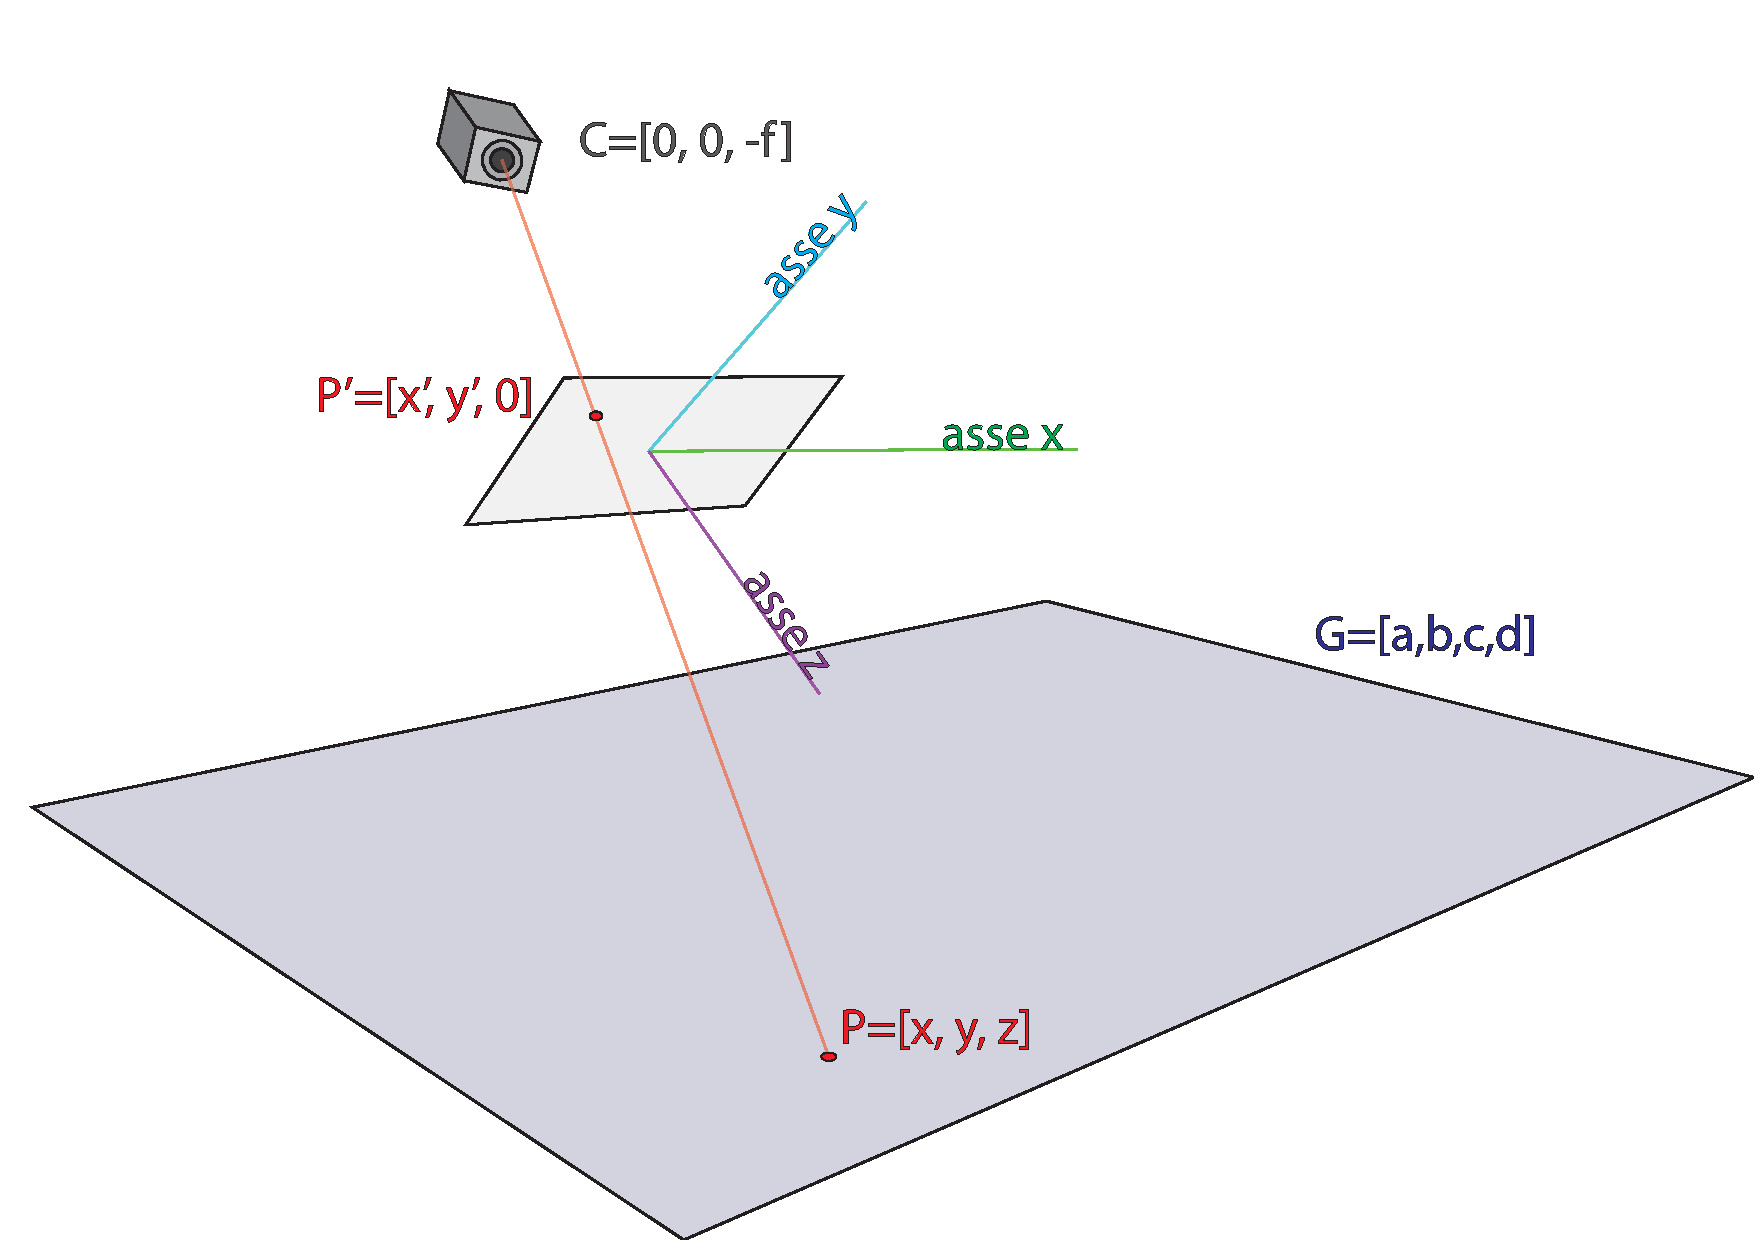
\includegraphics[width=\textwidth]{images/camera coords.pdf}
    \caption{Modello con coordinate}
    \label{fig:camera coords}
\end{figure}

Come espresso nella sezione \ref{sec:funzionalita-posizione} a noi interessa solamente ricorstruire ciò che accade sulla strada e ignoriamo il resto della scena.
Possiamo approssimare la strada con un piano, che chiamiamo piano stradale.
L'operazione che dobbiamo eseguire per correggere la distorsione prospettica si riduce così dalla proiezione da immagine a spazio reale tridimensionale a una proiezione da immagine a piano bidimensionale.
Questa operazione non è lineare in coordinate cartesiane, ma diventa lineare se si utilizzano coordinate proiettive omogenee, ed è quindi possibile definire una matrice lineare di trasformazione.

È possibile definire tale matrice direttamente, ma è anche possibile definirla come combinazione di trasformazioni.
Tutte le trasformazioni affini sono componibili in coordinate omogenee, ed abbiamo quindi accesso a traslazione, rotazione e scalatura, a cui aggiungiamo la trasformazione di proiezione.
La trasformazione di proiezione prende le coordinate di un punto sull'immagine e, date le coordinate del piano, restituisce la posizione reale del punto corrispondente al punto immagine.
Dato che le coordinate sono omogenee e non cartesiane, il punto immagine è espresso con 3 coordinate e il punto reale trovato con 4 coordinate.
La trasformazione di proiezione $P$ è rappresentata con la matrice \ref{eq:projmat}:
\begin{equation}
        \label{eq:projmat}
        P = 
        \begin{bmatrix}
            cf - d & 0      & 0   \\
            0      & cf - d & 0   \\
            -fa    & -fb    & -fd \\
            a      & b      & cf  \\
        \end{bmatrix}
\end{equation}
Dove:
\begin{itemize}
    \item il piano stradale è caratterizzato dall'equazione $ax + by + cz + d = 0$, oppure dal vettore $[a, b, c, d]^T$
    \item la lunghezza focale della camera è $f$
\end{itemize}

La matrice di trasformazione completa $M$ è definita quindi dalla combinazione di trasformazioni in \ref{eq:projcombo}:
\begin{equation}
    \label{eq:projcombo}
    M = D \cdot T \cdot R \cdot P
\end{equation}
Dove:
\begin{itemize}
    \item $P$ è la matrice di proiezione dall'immagine al piano
    \item $R$ è la rotazione dalla normale del piano all'opposto della normale dell'immagine
    \item $T$ è la traslazione dall'origine del piano all'origine dell'immagine
    \item $D$ è la matrice 
    $
    \begin{bsmallmatrix}
        1 & 0 & 0 & 0 \\
        0 & 1 & 0 & 0 \\
        0 & 0 & 0 & 1 \\
    \end{bsmallmatrix}
    $
    che scarta la coordinata $z$ e ci riporta da 3 dimensioni a 2 dimensioni
\end{itemize}
Ricordiamo che le trasformazioni combinano da destra verso sinistra.
Una rappresentazione visiva della combinazione è in fig \ref{fig:TODO}.

Diventa quindi possibile definire la matrice di correzione della distorsione prospettica in modo interattivo, manipolando la rotazione e la posizione della camera rispetto al piano stradale.
Possiamo infatti calcolare le coodinate del piano necessarie per $P$ partendo dal piano $[0, 0, 1, 0]$ (è il piano $z=0$) e applicando $R^{-1}$ e $T^{-1T}$ (la traslazione in coordinate proiettive si applica al piano mediante la trasposta della traslazione applicata ai punti).
In questo modo si può trovare una trasformazione soddisfacente, in cui le misure si avvicinano a quelle reali, senza i grandi costi implementativi richiesti dall'implementazione di un metodo automatico per la definizione del piano stradale.
Una volta definita la matrice di trasformazione il suo utilizzo risulta estremamente efficiente, in quanto si riduce a un prodotto matrice-vettore.

\begin{figure}
    \centering
    \begin{subfigure}{.49\textwidth}
        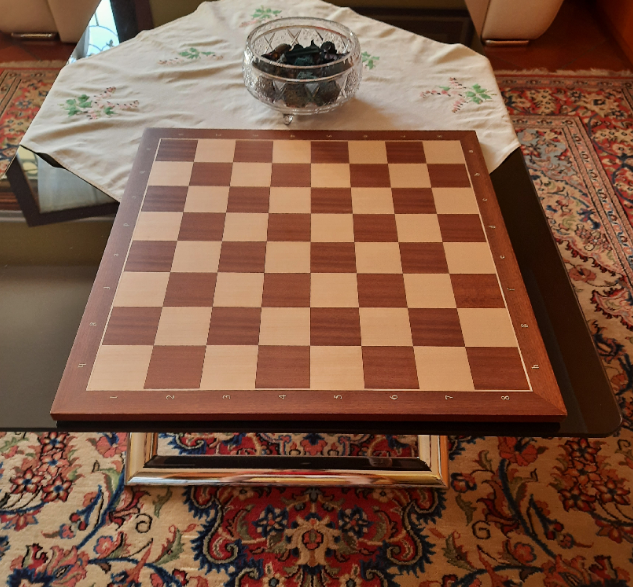
\includegraphics[width=\textwidth]{images/persp1.png}
    \end{subfigure}
    \hfill
    \begin{subfigure}{.49\textwidth}
        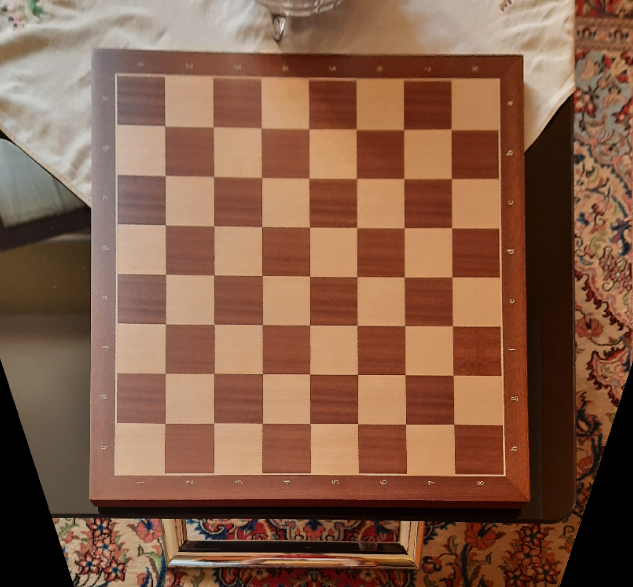
\includegraphics[width=\textwidth]{images/persp2.png}
    \end{subfigure}
    \caption{Esempio di correzione della distorsione prospettica}
    \label{fig:projcorrected}
\end{figure}

L'ultima considerazione necessaria è la scelta del punto a cui applicare la trasformazione trovata.
Notiamo dall'immagine \ref{fig:TODO} che scegliere il punto centrale del Bounding Box non restituisce il risultato desiderato.
La strategia migliore è quella di proiettare il lato inferiore del Bounding Box, in quanto questo è l'unico che poggia sul piano stradale.
Il centro delle entità può poi essere approssimato date le conoscenze relative a dimensioni medie della sua categoria, dalla sua direzione di movimento e dalle caratteristiche del Bounding Box.

In fig \ref{fig:perspyolo} è presentata una scena annotata dall'Object Detector Scaled-YoloV4 \cite{yolocsp}.
In fig \ref{fig:perspcorrect} è presentata la stessa scena dopo che è stata eseguita la correzione della distorsione prospettica, in cui la posizione dei veicoli è indicata dal cerchio verde.

\begin{figure}
    \centering
    \begin{subfigure}{.49\textwidth}
        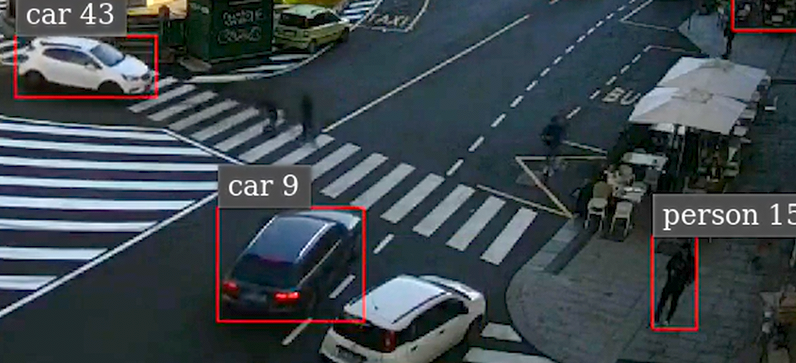
\includegraphics[width=\textwidth]{images/yolo.png}
        \caption{Scaled-YoloV4}
        \label{fig:perspyolo}
    \end{subfigure}
    \hfill
    \begin{subfigure}{.49\textwidth}
        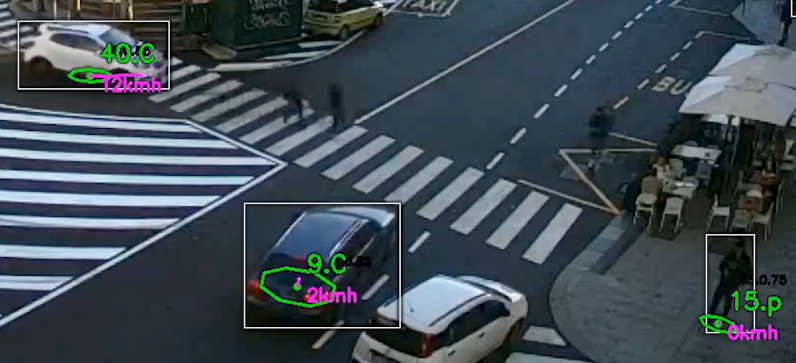
\includegraphics[width=\textwidth]{images/corrected.png}
        \caption{Distorsione corretta}
        \label{fig:perspcorrect}
    \end{subfigure}
    \caption{Scena prima e dopo la correzione della distorsione prospettica}
\end{figure}

\textbf{TODO: MANCANO 2 IMMAGINI}

\chapter{Velocità}
\label{sec:velocita}

Le misure ottenute fino ad ora presentano errori derivati dalla precisione non perfetta dell'Object Detection.
Potremmo pensare di  calcolare la velocità $V$ utilizzando l'equazione \ref{eq:vel}
\begin{equation}
    \label{eq:vel}
    \vec{V}_t = \frac{(\vec{P}_t - \vec{P}_{t-1})}{\Delta}
\end{equation}
dove $\vec{P}$ è la posizione reale calcolata in precedenza e $\Delta$ è intervallo tra $t$ e $t-1$.
Calcolare la velocità in questo modo amplifica però gli errori presenti nelle misure di posizione, soprattutto se $\Delta$ è piccolo, e restituisce misure non accettabili.
Possiamo però sfruttare il fatto che $\Delta$ è piccolo per affermare che la differenza tra $\vec{V}_t$ e $\vec{V}_{t-1}$ sia anch'essa piccola.
Possiamo quindi provare a correggere il rumore utilizzando una media mobile esponenziale, come in \ref{eq:ewma}
\begin{equation}
    \label{eq:ewma}
    \vec{V'}_t = k \cdot \vec{V'}_{t-1} + (1-k) \cdot \vec{V}_t
\end{equation}
dove $k \in [0, 1)$ e $V$ è calcolata come in \ref{eq:vel}.
Notiamo però che quest'approccio introduce un ritardo tra i valori calcolati e quelli reali (fig \ref{fig:lag}).
È perciò necessario utilizzare un algoritmo che corregga questo ritardo e allo stesso tempo corregga l'errore in modo simile alla media mobile.

\begin{figure}
    \centering
    \begin{subfigure}[b]{0.45\textwidth}
        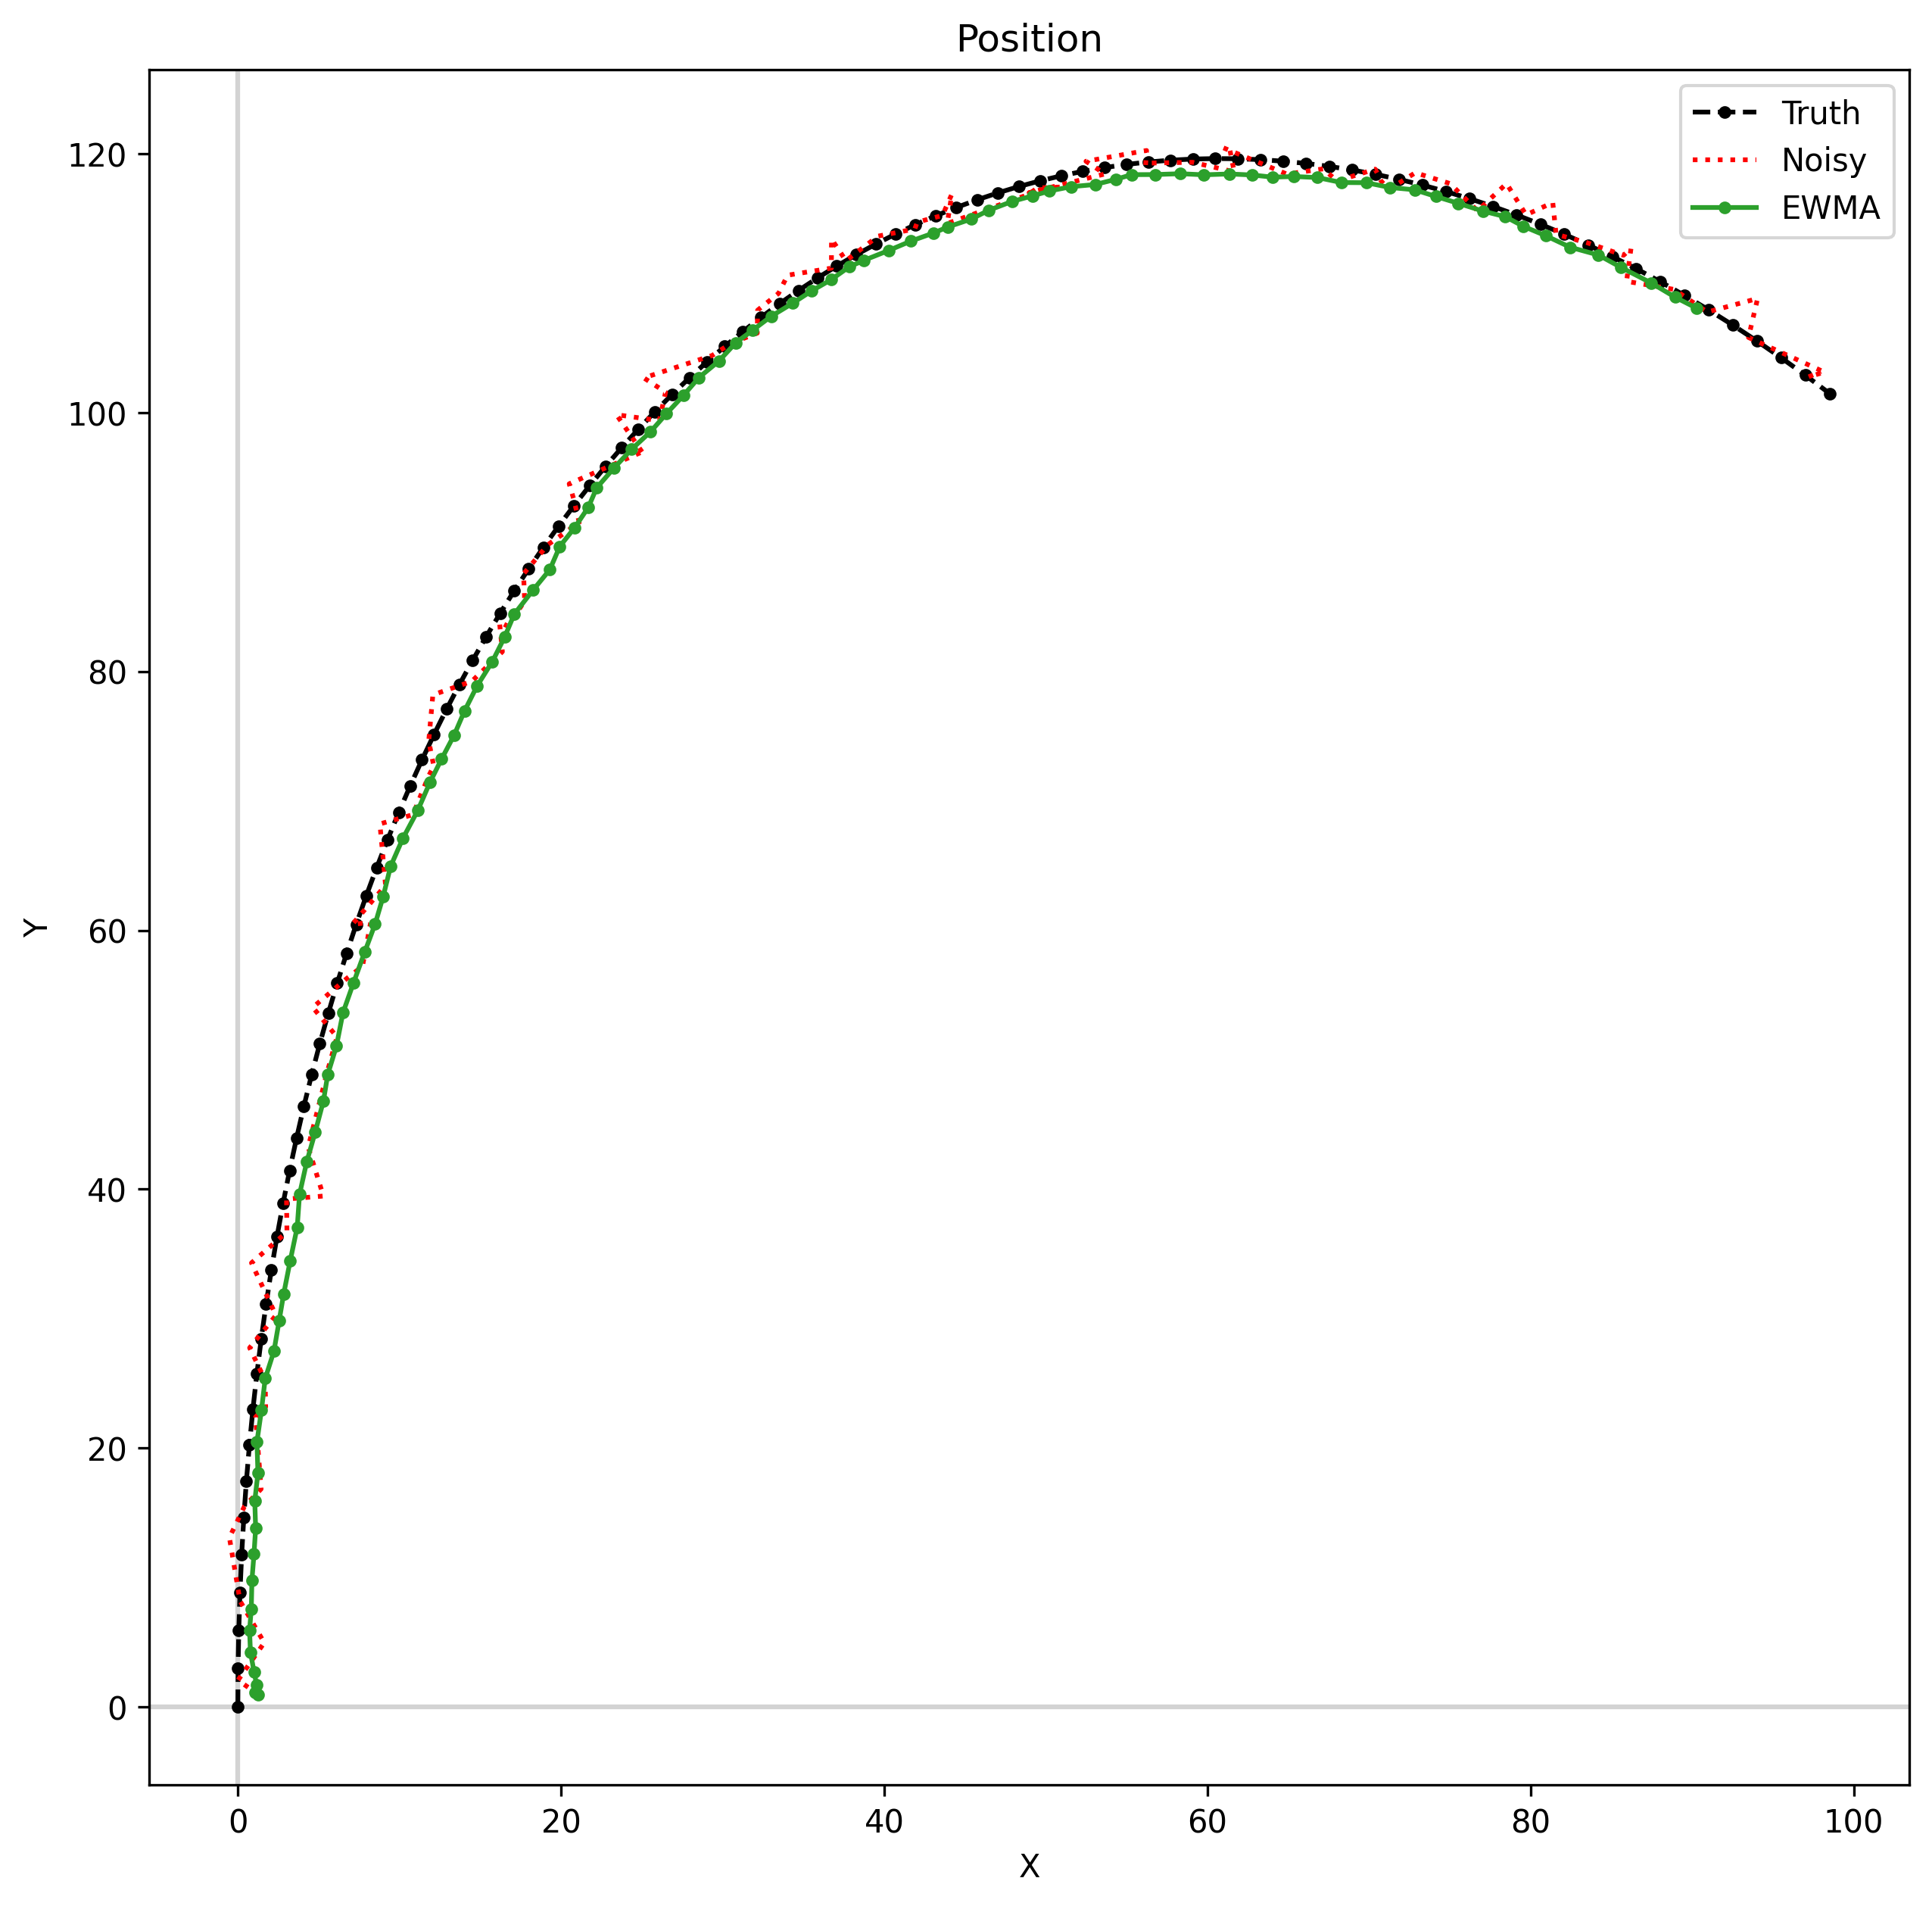
\includegraphics[width=\textwidth]{images/pos0.png}
        \caption{Posizione}
    \end{subfigure}
    \hfill
    \begin{subfigure}[b]{0.45\textwidth}
        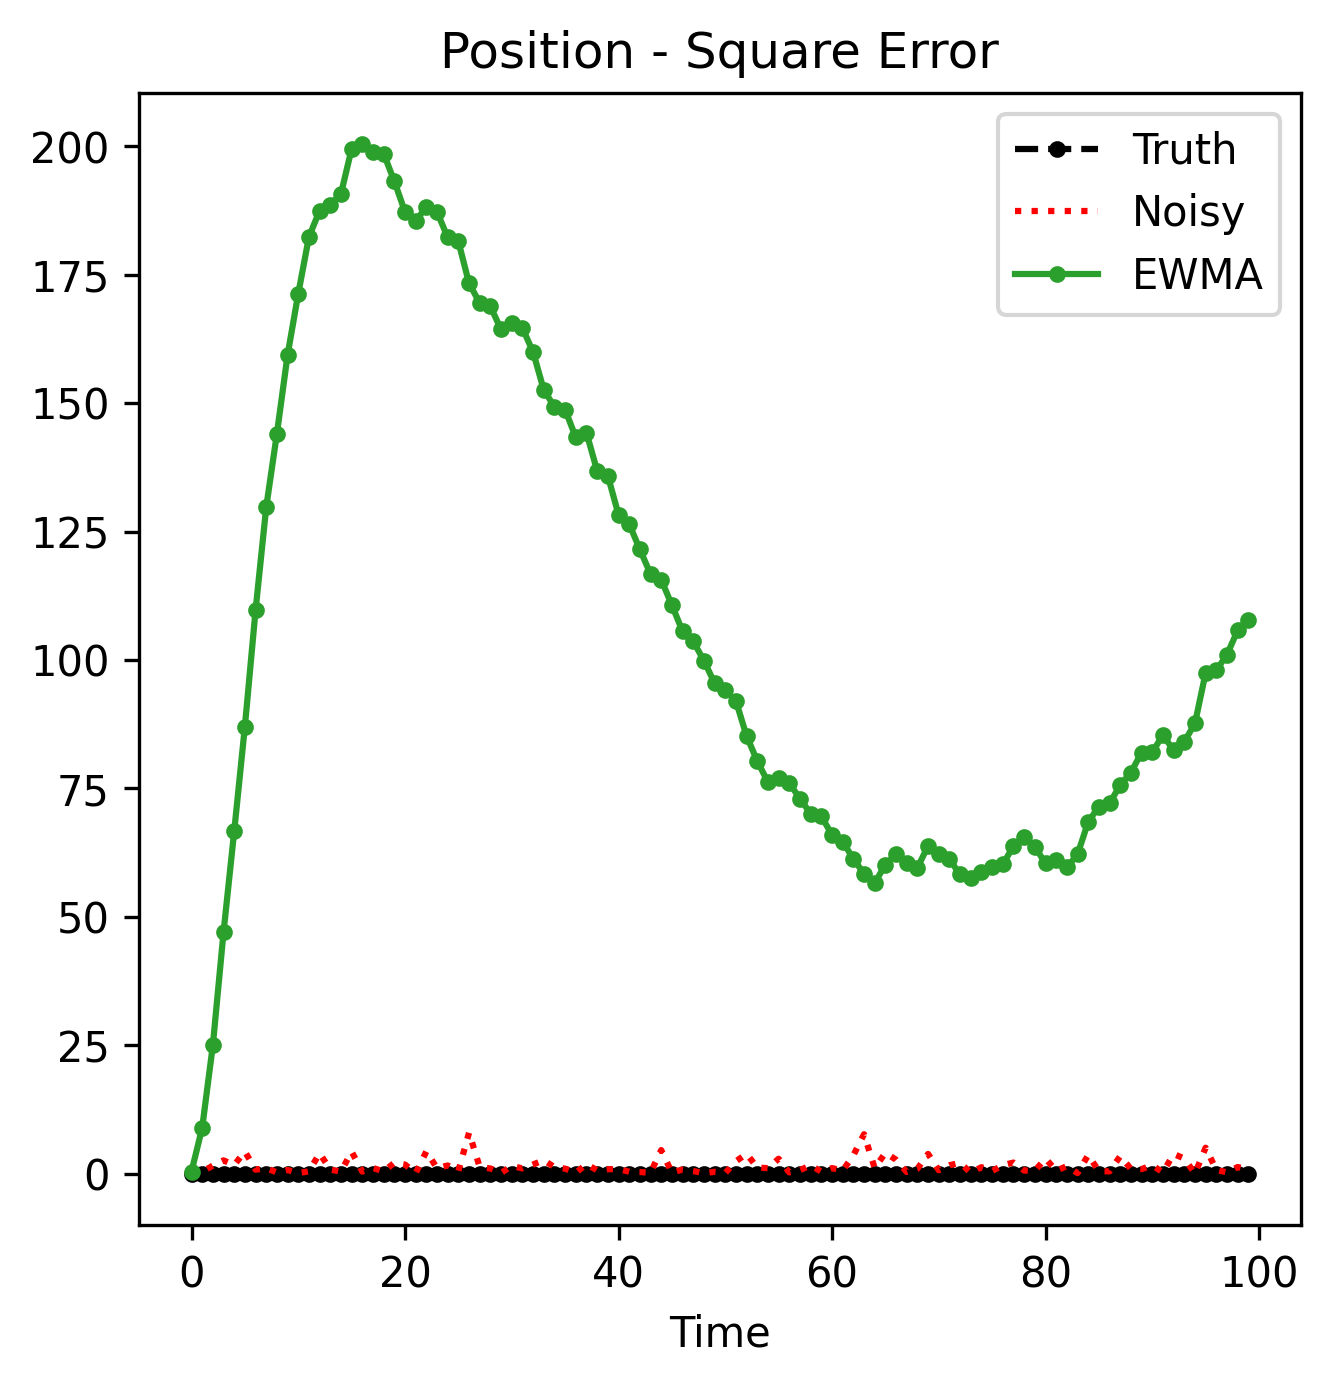
\includegraphics[width=\textwidth]{images/pos0err.png}
        \caption{Errore relativo alla posizione}
    \end{subfigure}
    \vfill
    \begin{subfigure}[b]{0.45\textwidth}
        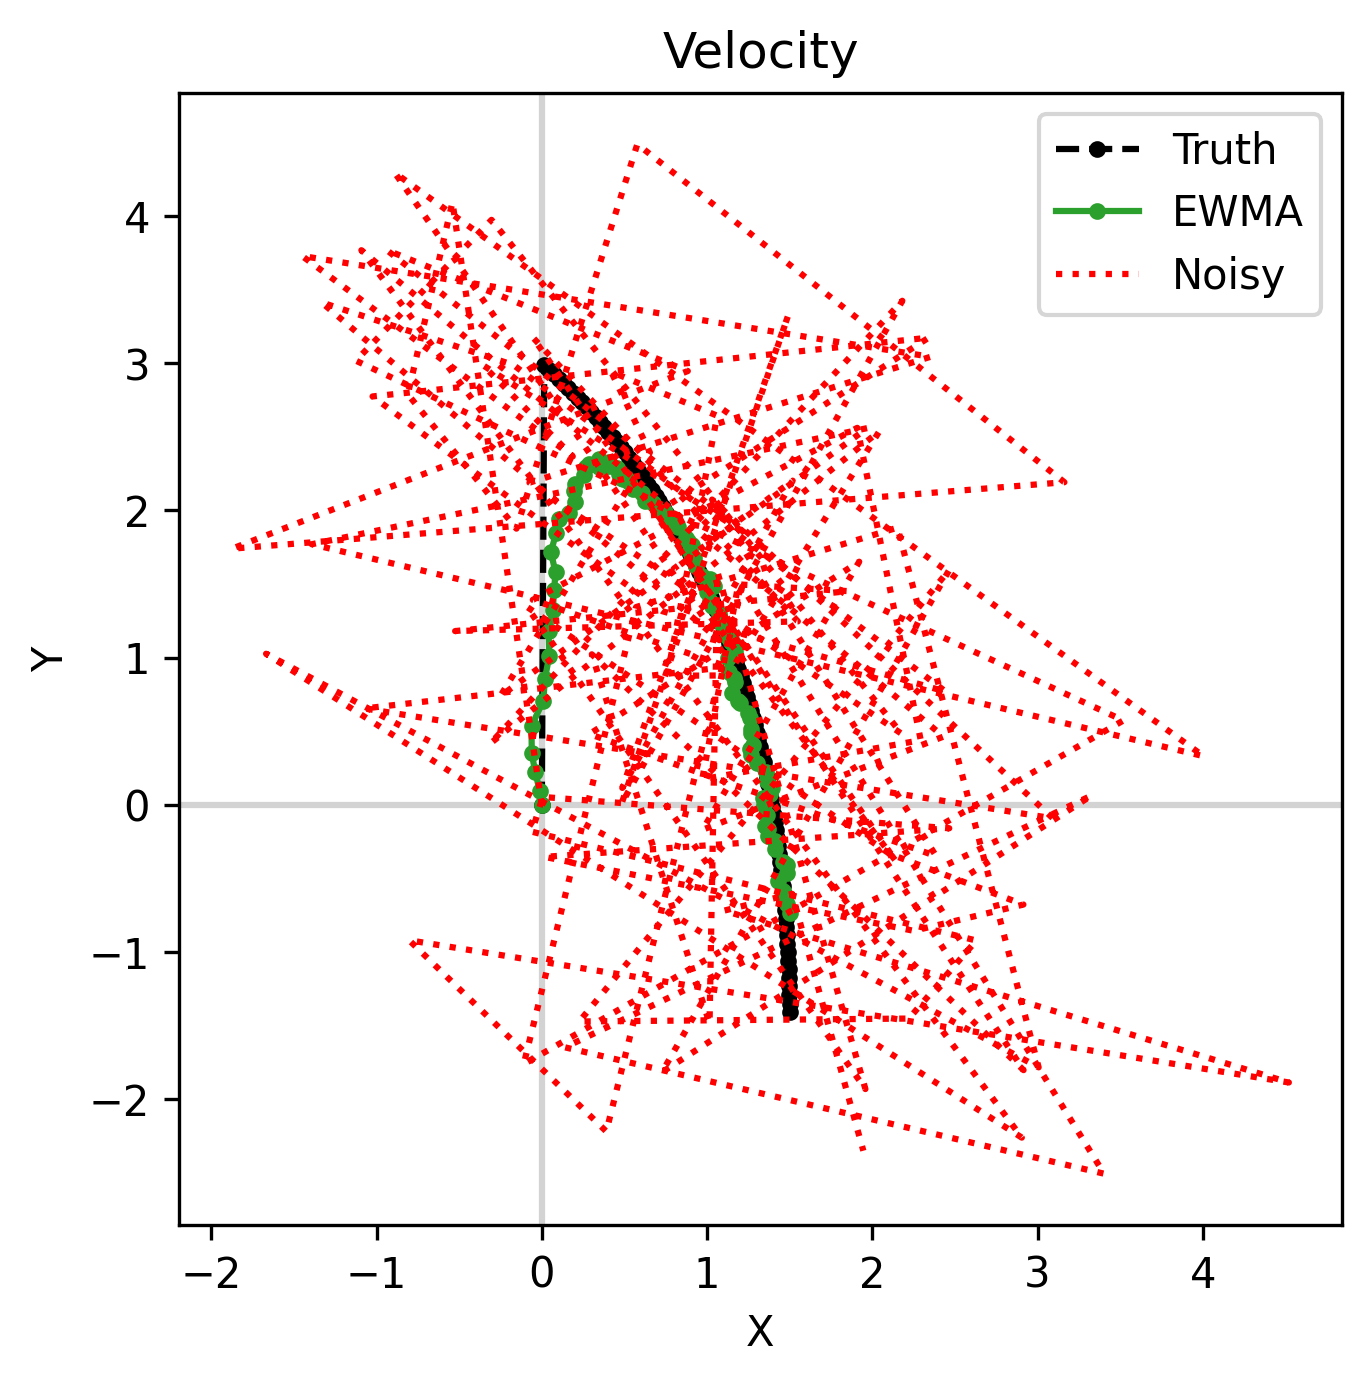
\includegraphics[width=\textwidth]{images/vel0.png}
        \caption{Velocità}
    \end{subfigure}
    \hfill
    \begin{subfigure}[b]{0.45\textwidth}
        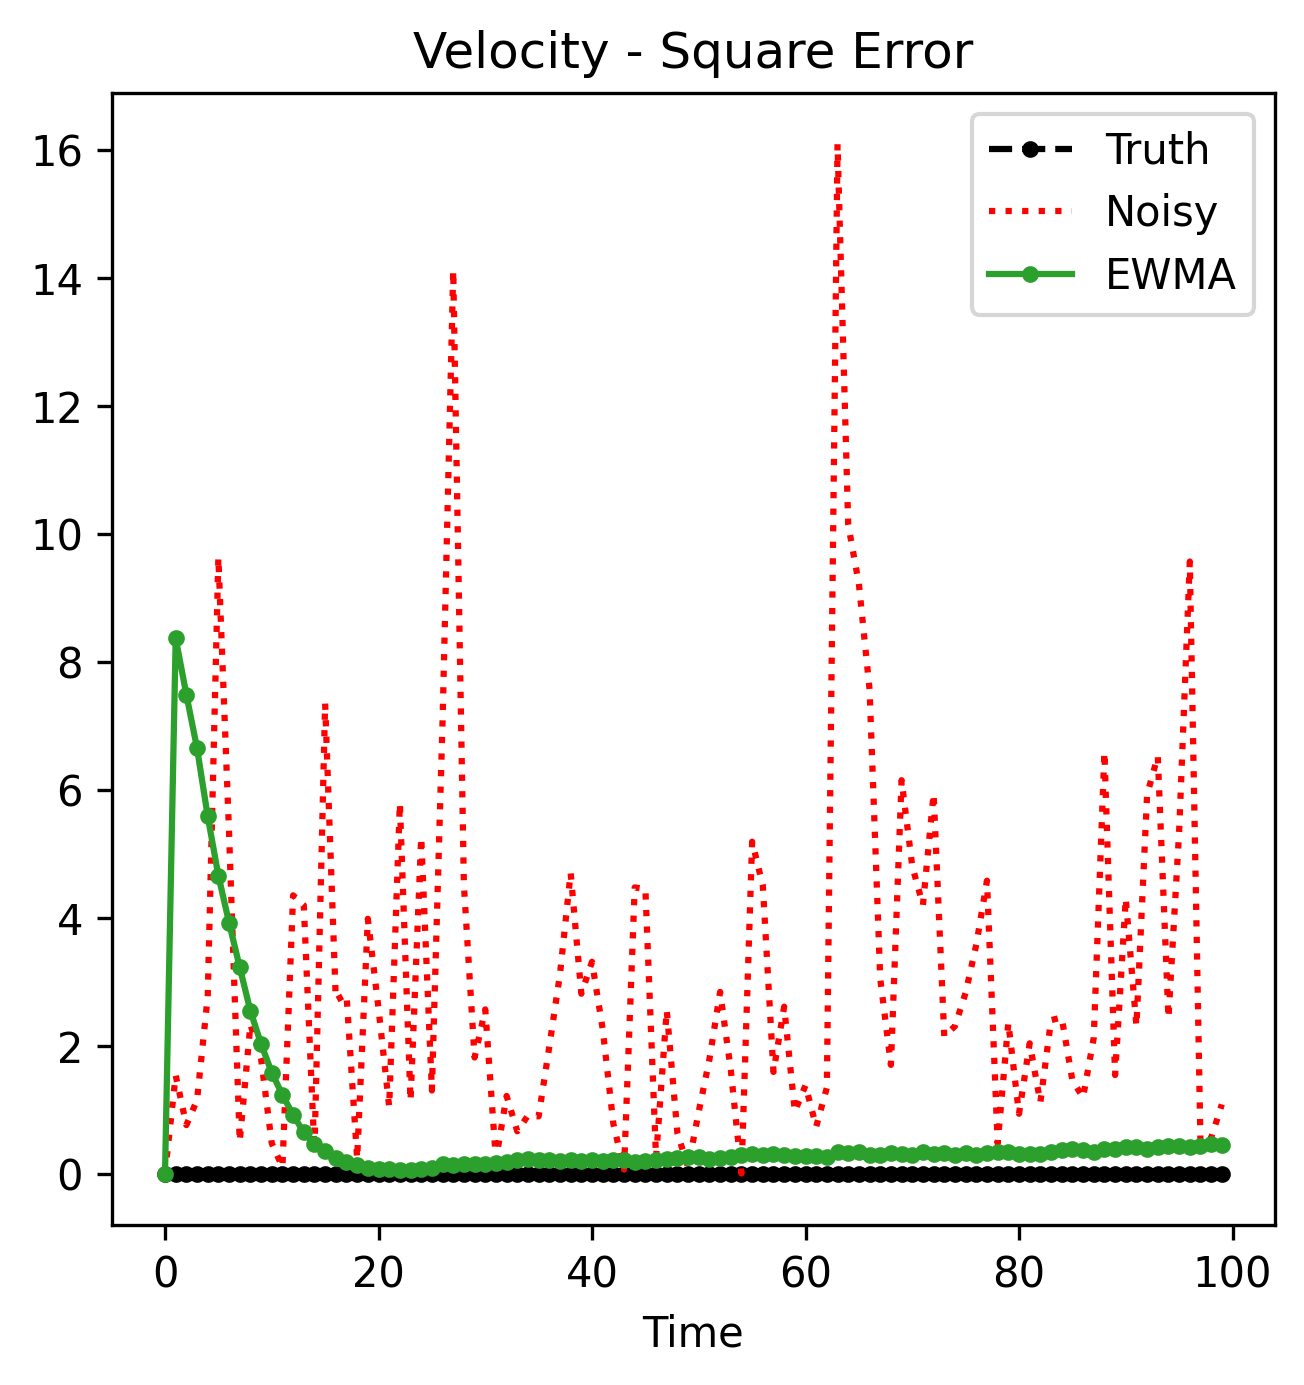
\includegraphics[width=\textwidth]{images/vel0err.png}
        \caption{Errore relativo alla velocità}
    \end{subfigure}
    \caption{Correggere il rumore utilizzando la media mobile esponenziale non restituisce risultati accettabili}
    \label{fig:lag}
\end{figure}

L'algoritmo da noi sviluppato è espresso dalle equazioni in \ref{eq:smoothns}
\begin{equation}
    \label{eq:smoothns}
    \begin{split}
        & p'_t = p_{t-1} + v_{t-1} + \frac{1}{2} \cdot a_{t-1} \\
        & v'_t = v_{t-1} + a_{t-1} \\
        & p_t = k \cdot p'_t + (1-k) \cdot P_t \\
        & v_t = k \cdot v'_t + (1-k) \cdot (p_t - p'_t) \\
        & a_t = k \cdot a_{t-1} + (1-k) \cdot (v_t - v'_t) \\
        & \\
        & P'_t = p_t + v_t \cdot \left(\frac{k}{1-k}\right) + \frac{1}{2} \cdot a_t \cdot \left(\frac{k}{1-k}\right)^2 \\
        & V'_t = 2 \cdot \left(v_t + a_t \cdot \left(\frac{k}{1-k}\right)\right)
    \end{split}
\end{equation}
\begin{itemize}
    \item $k \in [0, 1)$ è il coefficiente di correzione
    \item $P_t$ è la posizione osservata all'istante $t$
    \item $p'_t$ è la statistica posizione che ci aspettiamo di avere in base alle nostre conoscenze
    \item $v'_t$ è la statistica velocità che ci aspettiamo di avere in base alle nostre conoscenze
    \item $p_t$ è la statistica relativa alla posizione all'istante $t$
    \item $v_t$ è la statistica relativa alla velocità all'istante $t$
    \item $a_t$ è la statistica relativa all'accelerazione all'istante $t$
    \item $P'_t$ è la posizione corretta all'istante $t$
    \item $V'_t$ è la velocità corretta all'istante $t$
\end{itemize}

Per valutare l'algoritmo sviluppato lo abbiamo messo a confronto con l'algoritmo pubblicato da J.LaViola in \cite{laviola}.
Questo algoritmo è espresso dalle equazioni in \ref{eq:laviola}
\begin{equation}
    \label{eq:laviola}
    \begin{split}
        & Sp_t = \alpha \cdot P_t + (1-\alpha) \cdot Sp_{t-1} \\
        & Sp^{[2]}_t = \alpha \cdot Sp_{t} + (1-\alpha) \cdot Sp^{[2]}_{t-1} \\
        & P'_T = \left(2 + \frac{\alpha \cdot \tau}{1 - \alpha}\right) \cdot Sp_t - \left(1 + \frac{\alpha \cdot \tau}{1 - \alpha}\right) \cdot Sp^{[2]}_t \\
    \end{split}
\end{equation}
\begin{itemize}
    \item $\alpha \in [0, 1)$ è il coefficiente di correzione
    \item $P_t$ è la posizione osservata all'istante $t$
    \item $Sp_t$ è la prima statistica relativa alla posizione all'istante $t$
    \item $Sp^{[2]}_t$ è la seconda statistica relativa alla posizione all'istante $t$
    \item $P'_T$ è la posizione corretta all'istante $T$
    \item $\tau = T - t$ ci permette di predirre la posizione anche in istanti futuri. Nel nostro caso d'uso è sempre uguale a 0.
\end{itemize}
I coefficienti di correzione sono correlati dall'equazione $\alpha = 1-k$.
Il confronto proposto è eseguito con le seguenti condizioni:
\begin{itemize}
    \item $k := 0.85$
    \item $v_0 := a_0 := Sp^{[2]}_0 := [0, 0]$
    \item $p_0 := Sp_0 =: P_0$
    \item Il percorso reale è generato attraverso una curva di Bezier con estremità $[0, 0], [100, 100]$ e punti di controllo $[0, 100], [100, 0]$
    \item Il numero di intervalli è $100$
\end{itemize}
Entrambi gli algoritmi lavorano ad intervalli discreti, e suppongono che le osservazioni siano ad intervalli costanti.
Entrambi correggono la posizione delle entità, e mentre il nostro permette di estrarre in contemporanea informazioni relative alla velocità, per ricavare la velocità dall'altro algoritmo è necessario utilizzare l'equazione \ref{eq:vel} e riapplicare l'algoritmo sui risultati.

\begin{figure}
    \centering
    \begin{subfigure}[b]{0.49\textwidth}
        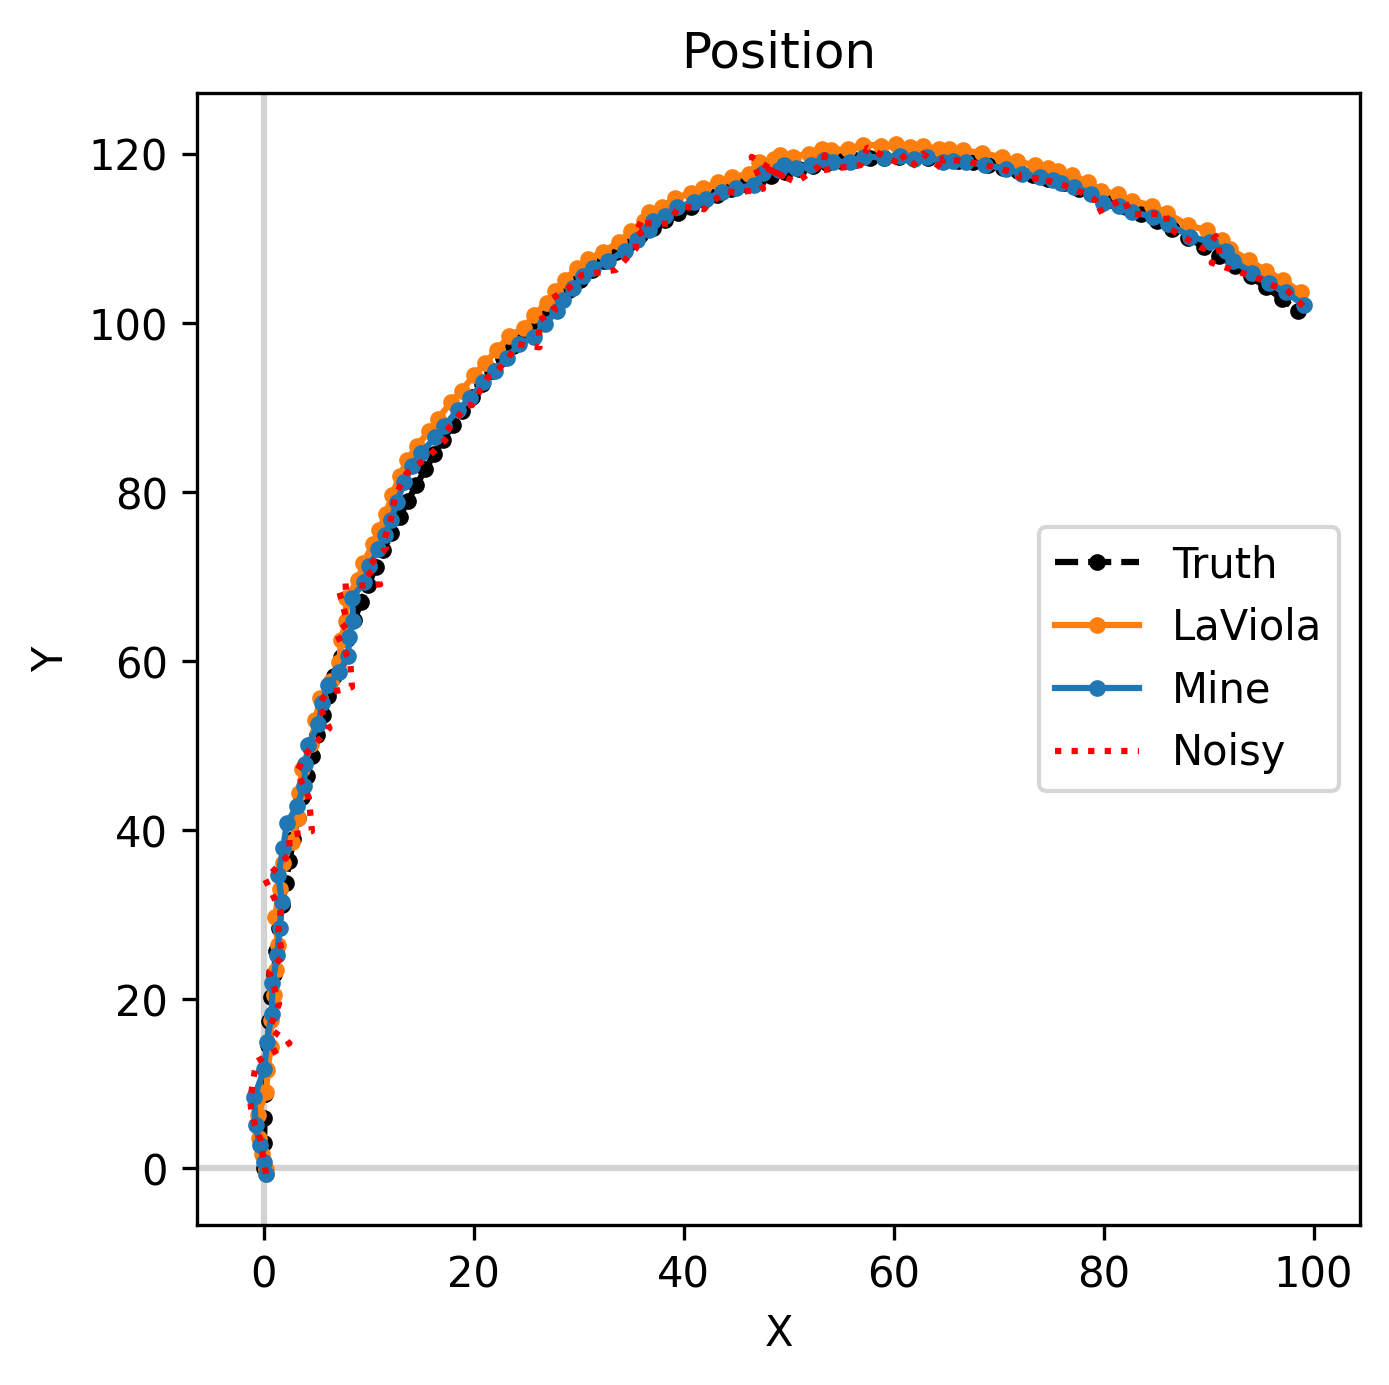
\includegraphics[width=\textwidth]{images/pos1.png}
        \caption{Posizione}
    \end{subfigure}
    \hfill
    \begin{subfigure}[b]{0.49\textwidth}
        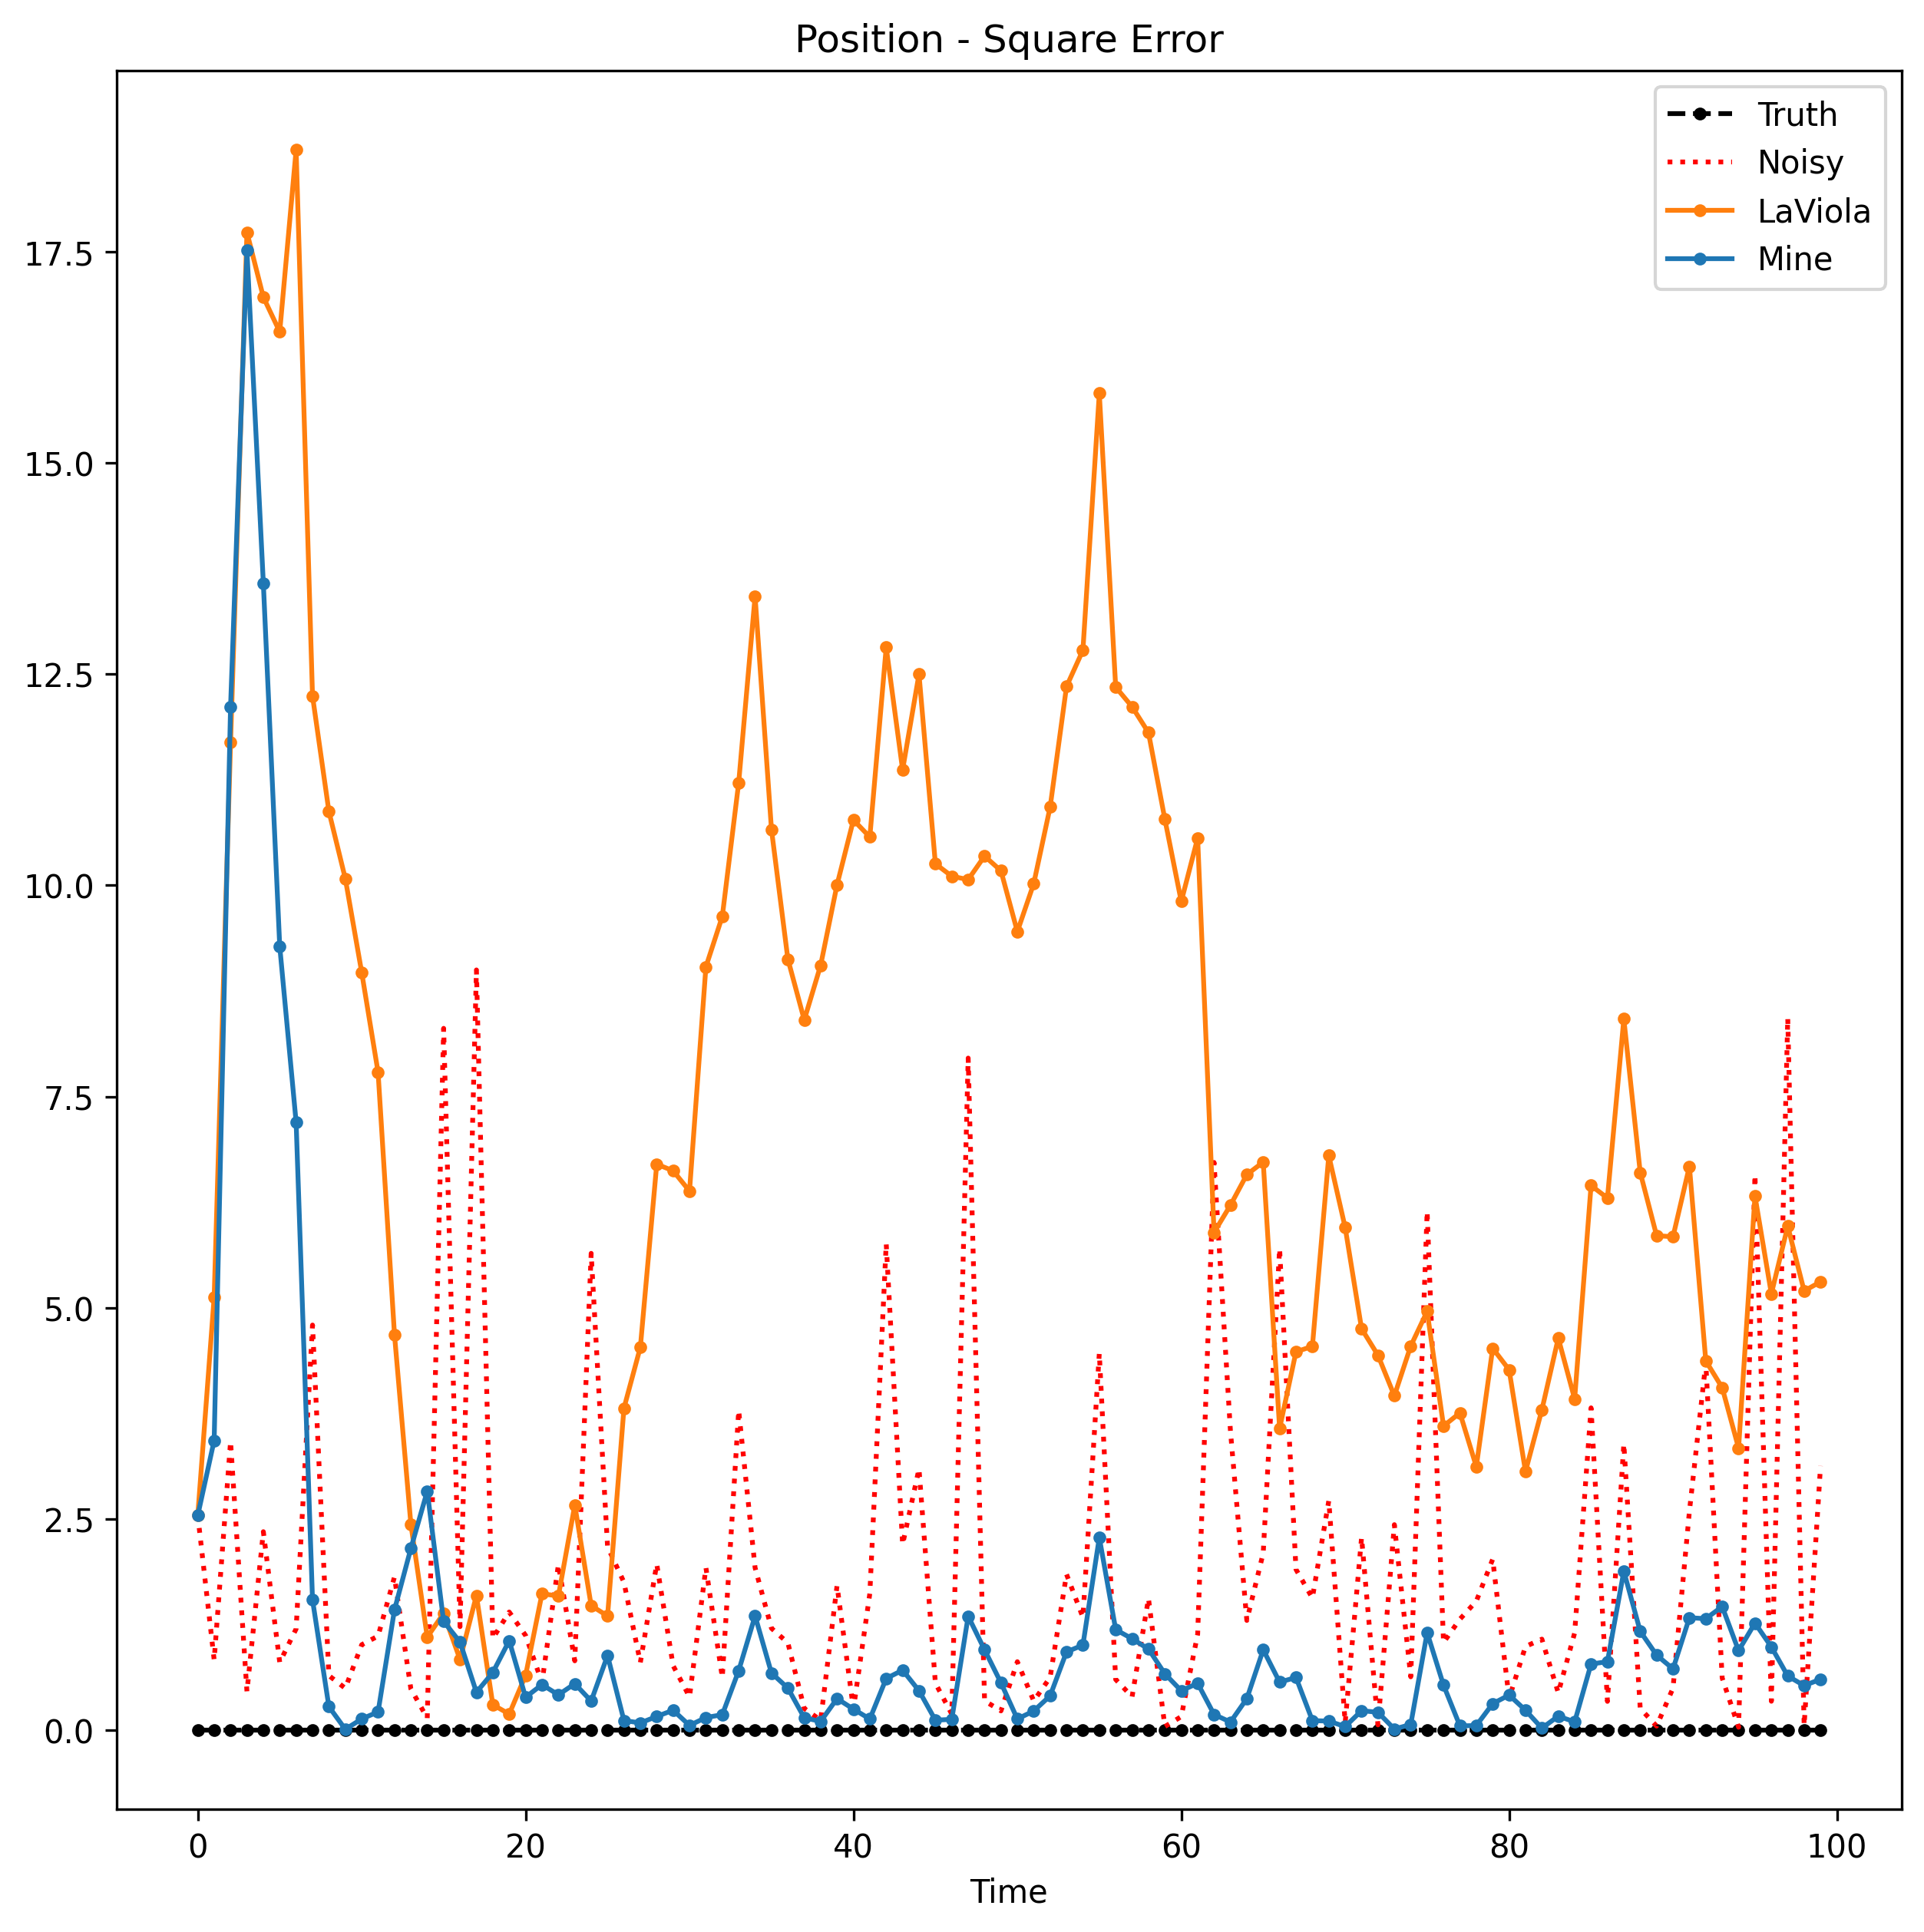
\includegraphics[width=\textwidth]{images/pos1err.png}
        \caption{Errore relativo alla posizione}
    \end{subfigure}
    \caption{Correzione della posizione}
    \label{fig:corrpos}
\end{figure}

\begin{table}
    \caption{Posizione: Errore quadrato medio}
    \label{tab:peqm}
    \centering
    \begin{subtable}{.49\textwidth}
        \caption{da $t=0$}
        \centering
        \begin{tabular}{l r}
            Rumore &    1.5255 \\
            EWMA &    107.4193 \\
            LaViola &   5.3685 \\
            Nostro &    1.2400 \\
        \end{tabular}
    \end{subtable}
    \hfill
    \begin{subtable}{.49\textwidth}
        \caption{ da $t=20$ }
        \label{tab:peqmb}
        \centering
        \begin{tabular}{l r}
            Rumore &   1.5578 \\
            EWMA &   100.6619 \\
            LaViola &  2.3364 \\
            Nostro &   0.5000 \\
        \end{tabular}
    \end{subtable}
\end{table}

\begin{figure}
    \begin{subfigure}[b]{0.49\textwidth}
        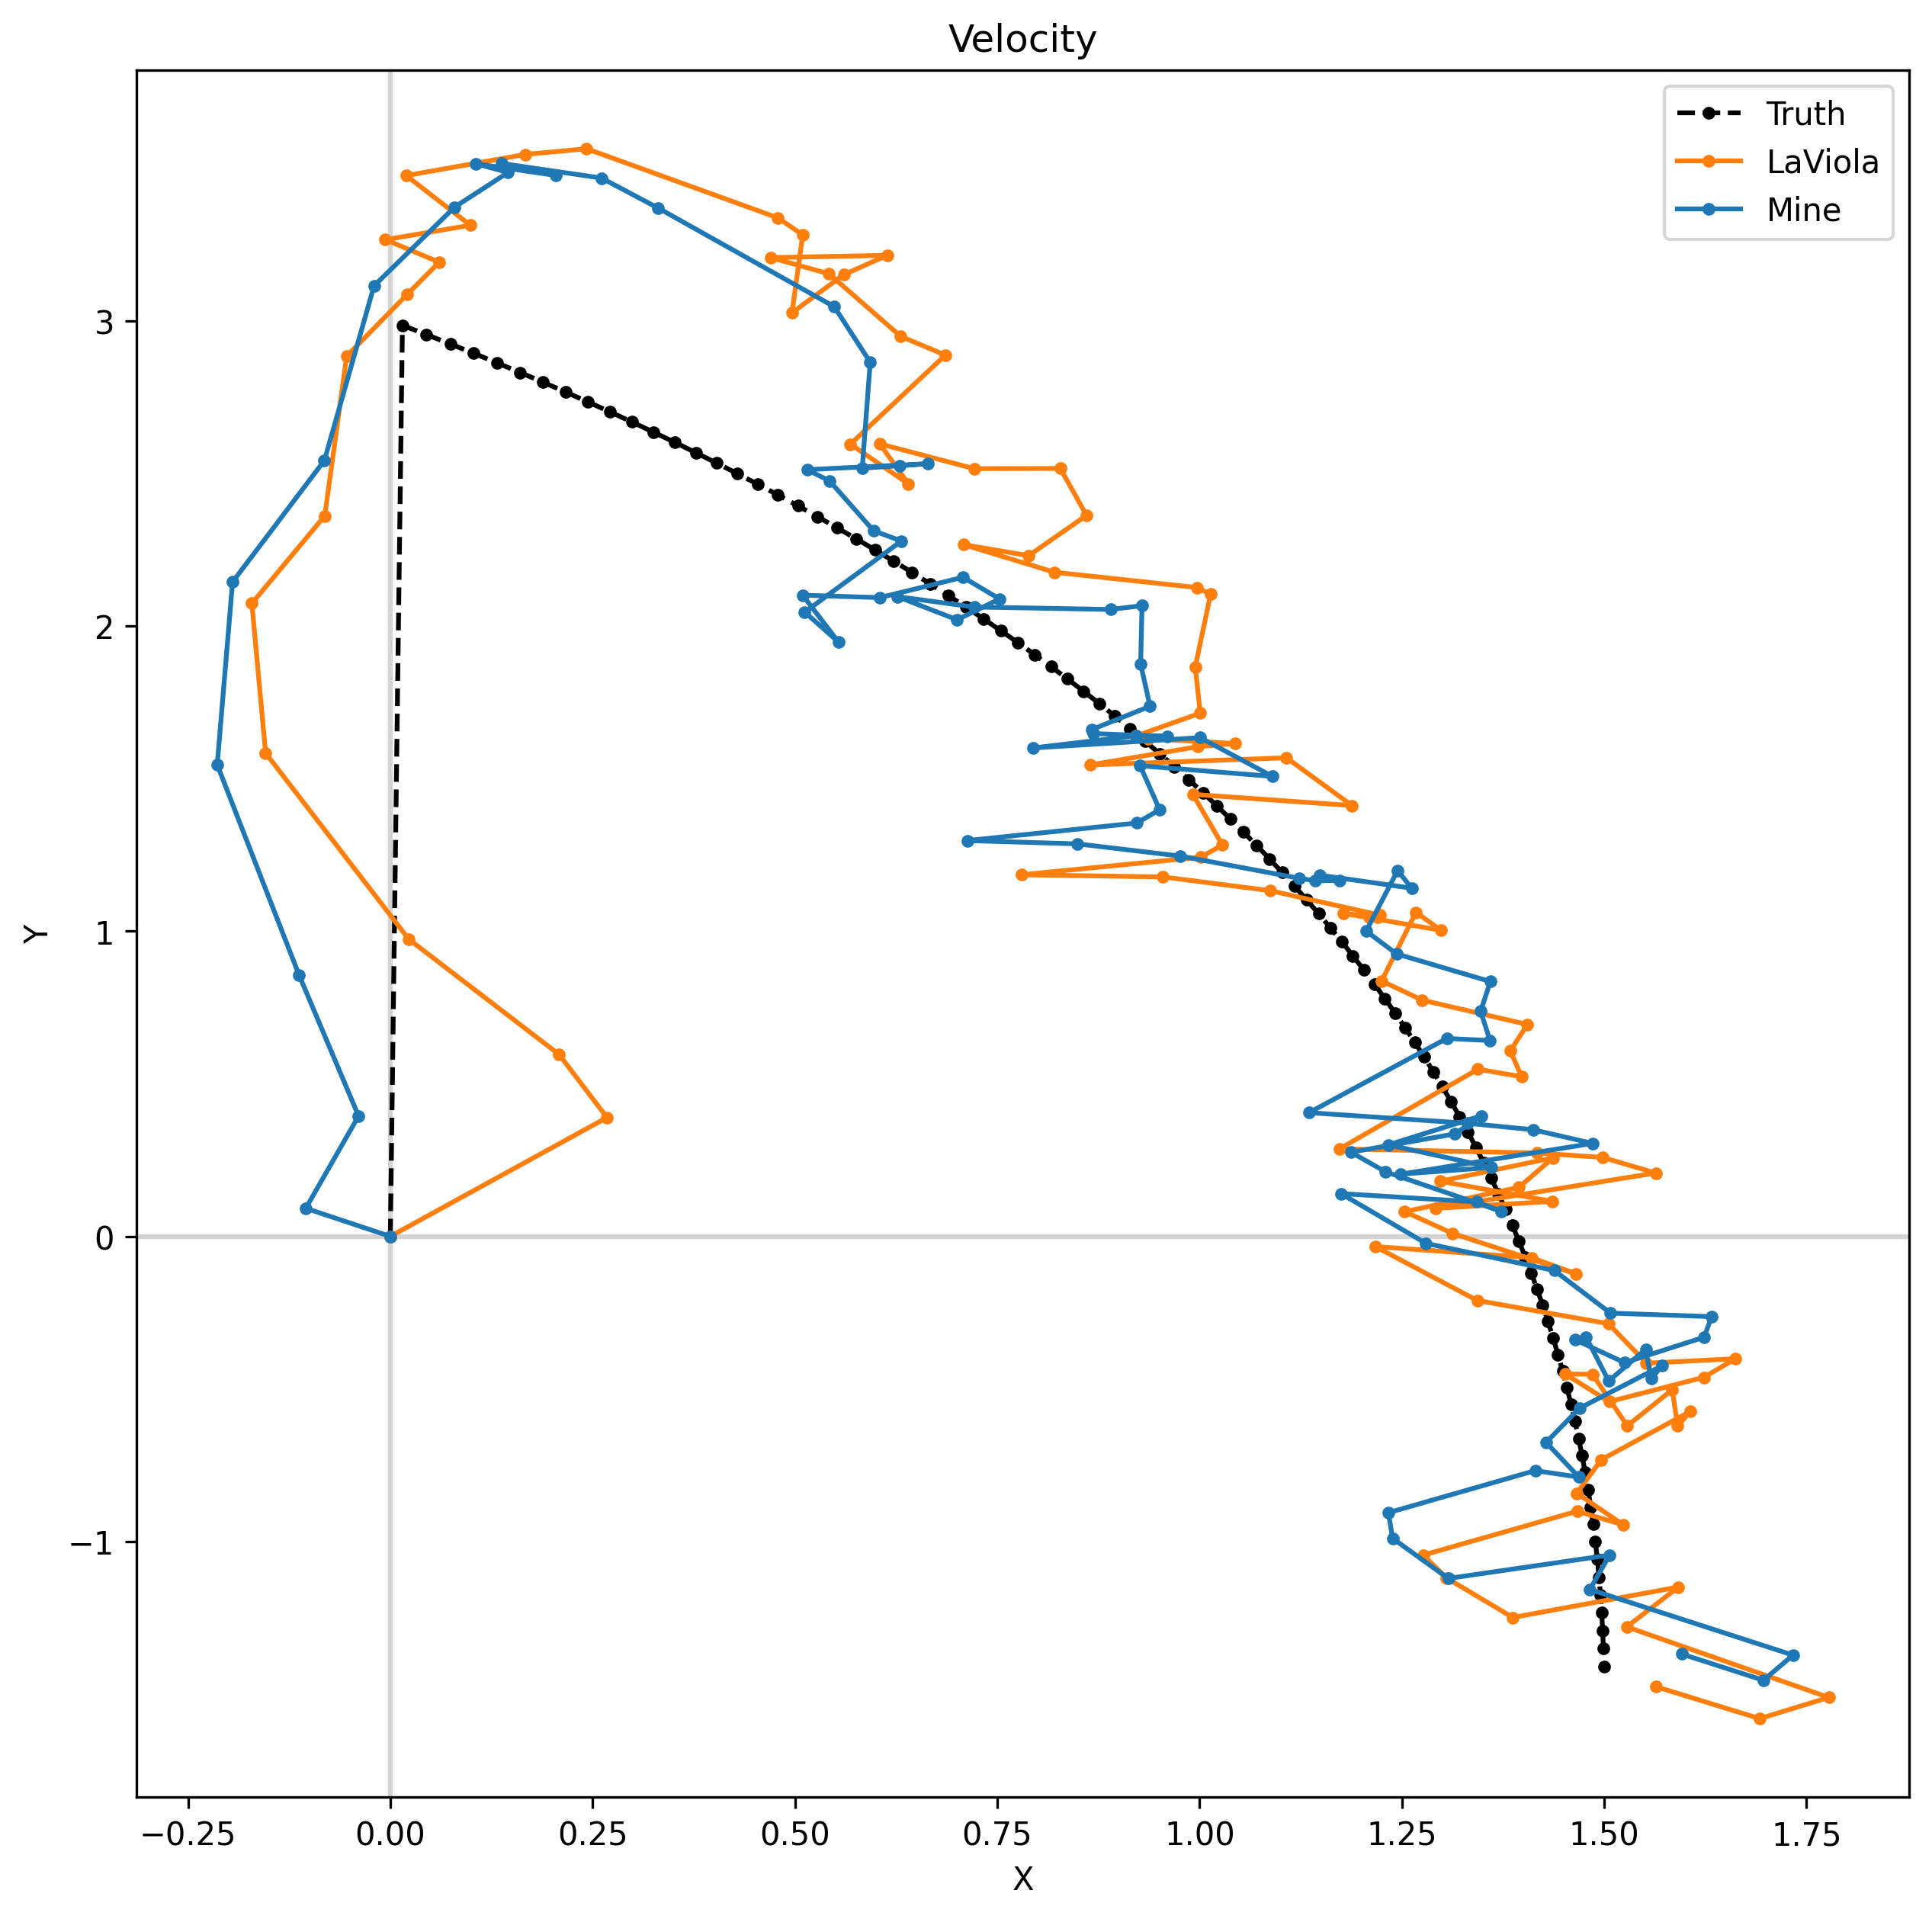
\includegraphics[width=\textwidth]{images/vel1.png}
        \caption{Velocità}
    \end{subfigure}
    \hfill
    \begin{subfigure}[b]{0.49\textwidth}
        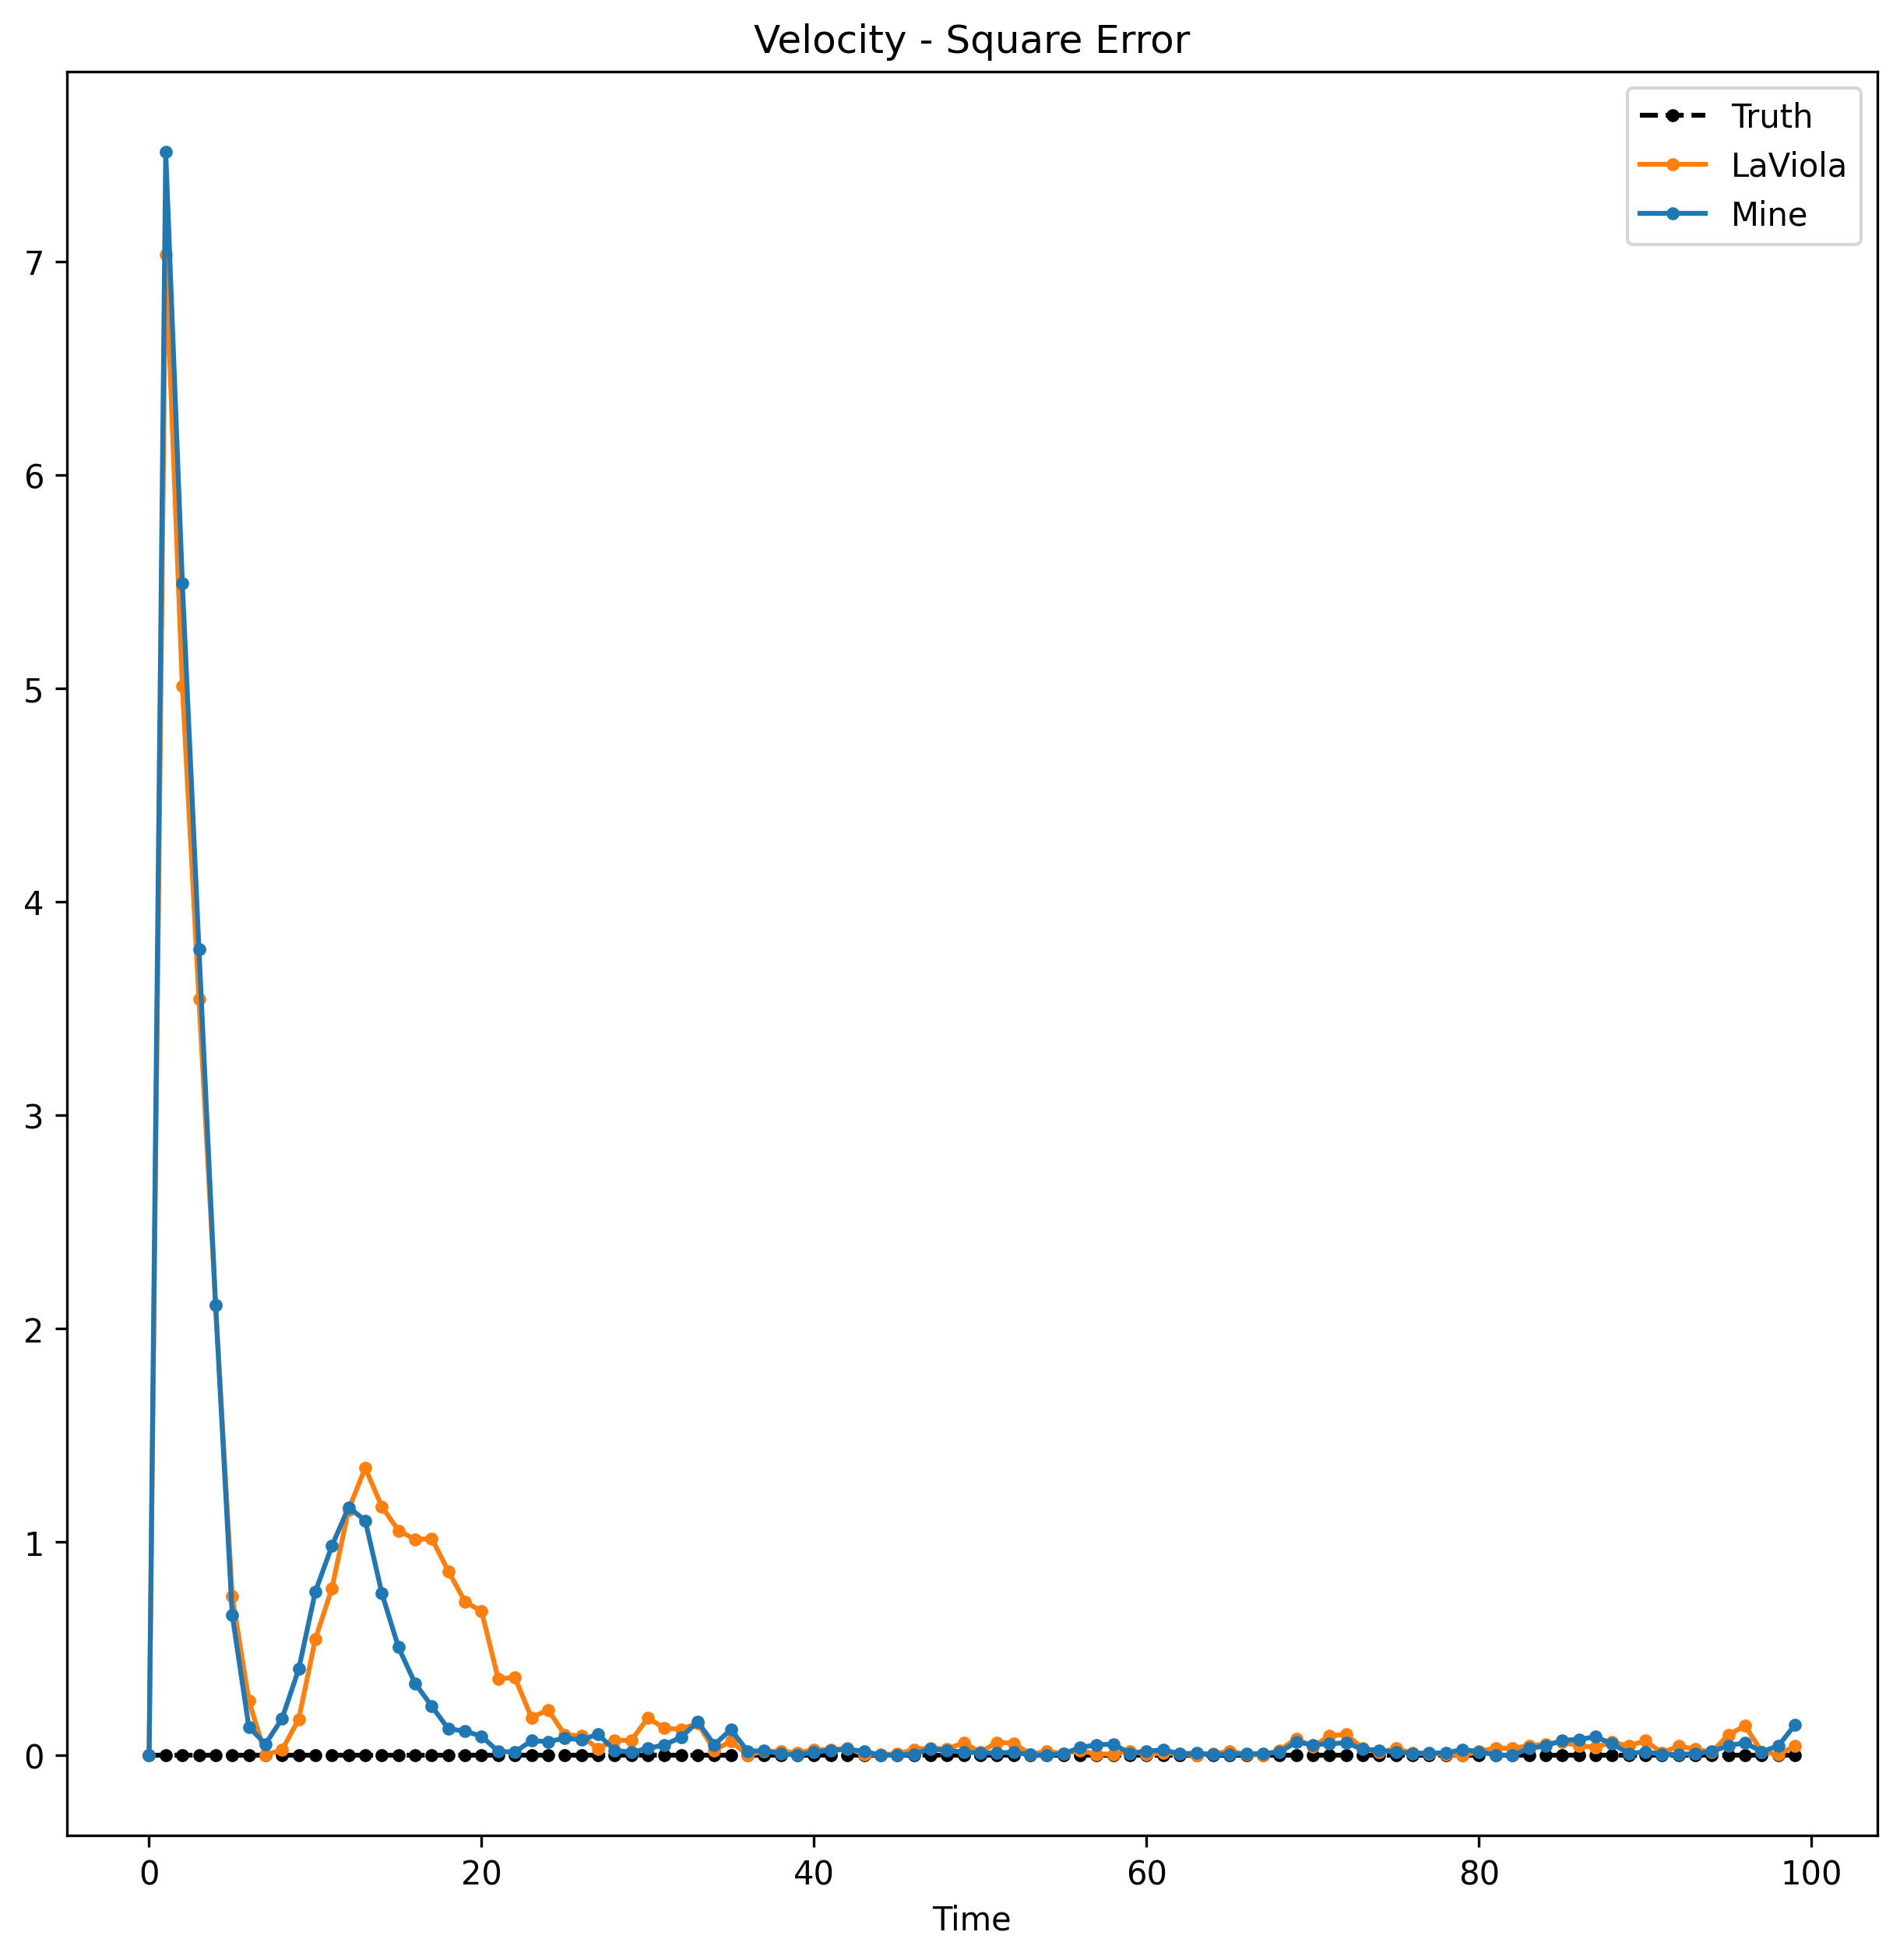
\includegraphics[width=\textwidth]{images/vel1err.png}
        \caption{Errore relativo alla velocità}
    \end{subfigure}
    \caption{Correzione della velocità}
    \label{fig:corrvel}
\end{figure}

\begin{table}
    \caption{Velocità: Errore quadrato medio}
    \label{tab:veqm}
    \centering
    \begin{subtable}{.49\textwidth}
        \caption{da $t=0$}
        \centering
        \begin{tabular}{l r}
            Rumore  & 3.0807 \\
            EWMA    & 0.7228 \\
            LaViola & 0.2980 \\
            Nostro  & 0.2397 \\
        \end{tabular}
    \end{subtable}
    \hfill
    \begin{subtable}{.49\textwidth}
        \caption{ da $t=20$ }
        \label{tab:veqmb}
        \centering
        \begin{tabular}{l r}
            Rumore  & 3.1961 \\
            EWMA    & 0.2744 \\
            LaViola & 0.0484 \\
            Nostro  & 0.0267 \\
        \end{tabular}
    \end{subtable}
\end{table}

L'errore indicato nelle tabelle \ref{tab:peqm} e \ref{tab:veqm} è l'errore quadrato assoluto.
Le alte punte ad inizio esecuzione sono legate all'inizializzazione dei valori dell'algoritmo.
Se inizializzassimo $v$ e $a$ con valori migliori potremmo ridurre gli errori in fase di sincronizzazione e ottenere risultati simili a \ref{tab:peqmb} e \ref{tab:veqmb} sin da inizio esecuzione.
Dai risultati ottenuti si può verificare che il nostro algoritmo ottiene risultati almeno comparabili a quelli ottenuti dell'algoritmo di confronto.
Questo ci da la sicurezza di aver sviluppato un algoritmo corretto e utile, ma valutazioni conclusive sulla sua qualità richiedono test più profondi e confronti con algoritmi diversi.
In particolare sarebbe interessante un confronto con algoritmi basati su Kalman Filter e sue estensioni. 

\chapter{Architettura}
\label{sec:architettura}

% TODO: AGGIUNGI IMMAGINI, RIFERIMENTI 

% Definire e desccrivere nei dettagli l'architettura a blocchi, descrivendo ciascun blocco e i collegamenti.
% Non è ancora necessario dare dettagli implementativi, che andranno nel capitolo dedicato.
% Descrizione tecnologie utilizzate per implementare ciascun blocco.
% Qui vanno i dettagli implementativi per ciascun blocco dell'architettura definita nel capitolo precedente.
% Potrebbe convenire replicare l'immagine dell'architettura, definendo all'interno dell'immagine dettagli implementativi come ad esempio i nomi dei moduli utilizzati e le tecnologie utilizzate per implementarli.

\textbf{TODO: AGGIUNGI IMMAGINE}

L'architettura scelta è una pipeline, in quanto l'input del sistema è uno stream video.
Ogni frame dello stream deve essere processato nello stesso modo, e utilizzare una pipeline consente di aggiungere, rimuovere o sostituire moduli, e quindi modificare il processo, in modo semplice e veloce.

Il sistema è implementato sul dispositivo \emph{Nvidia Jetson Xaxier}\cite{arch:jetson} ed è sviluppato su \emph{Ubuntu 18.04}\cite{arch:ubuntu}.
Il linguaggio di sviluppo è \emph{Python 3.6}\cite{arch:python}.
Per la gestione delle operazione di algebra lineare sono stati utilizzati i package \emph{Numpy}\cite{arch:numpy} e \emph{SciPy}\cite{arch:scipy}.
La pipeline di acquisizione è gestita dalla libreria \emph{GStreamer}\cite{arch:gstreamer}.
La classificazione è effettuata dal modulo di inferenza fornito dall'\emph{SDK Nvidia Deepstream}\cite{arch:deepstream}.
Questo modulo di inferenza è configurato per il modello di \emph{Object Detection Scaled--YoloV4}\cite{yolocsp}.
Il tracking è gestito dal tracker \emph{NvDCF} \cite{nvdcf}, anch'esso fornito dall'\emph{SDK Nvidia Deepstream}.
La segnalazione delle anomalie è effettuata utilizzando la libreria \emph{Requests} \cite{arch:requests}.

\chapter{Conclusioni}
\label{sec:conclusioni}

L'obiettivo iniziale di correggere la \emph{distorsione prospettica} presente nelle misure di posizione e velocità è stato perciò raggiunto.
Questo risultato è stato ottenuto modellando il problema matematicamente in modo da comprendere la natura della distorsione e da individuare le approssimazioni necessarie alla sua risoluzione.
La fase complicata si è rivelata essere la generazione della trasformazione correttiva e non la sua applicazione.
È stato perciò necessario sviluppare uno strumento esterno interattivo con cui semplificare tale generazione.
Il lavoro fatto è stato poi validato confrontando i risultati ottenuti dal sistema di rilevazione di anomalie prima e dopo l'implementazione della soluzione proposta.

Possibili sviluppi futuri della soluzione trovata sono il permettere la definizione di trasformazioni sulla stessa immagine, in modo da gestire ambienti in cui un singolo piano non rende un'approssimazione soddisfacente.
Inoltre potrebbe essere interessante implementare i metodi discussi nella sezione riguardante lo stato dell'arte (Capitolo \ref{sec:introduzione}) nello strumento interattivo, come supporto all'operatore.

% NON SUDDIVISA per punti ma discorsiva (io suddivido per punti per chiarezza):
% •	l'obiettivo era (notare il tempo al passato) bl bla ripeti quanto detto in cap 1
% •	Abbiamo perseguito gli scopi preposti facendo bla bla ribadisci quanto raccontato nella tesi
% •	I risultati sono bla bla (sottolinea le cose + salienti
% •	commenti, limiti del lavoro, considerazioni, conclusioni e sviluppi futuri.


\pagestyle{empty}

\chapter*{Ringraziamenti}
Ringrazio il Dott. Sebastian Podda per ...

Ringrazio il Prof. Salvatore Carta per ...

Ringrazio infine la mia famiglia per ...


\addcontentsline{toc}{chapter}{Ringraziamenti}%

\bibliographystyle{splncs04}
\bibliography{bibliography}

\nocite{*}



% ----------------- ELENCO DELLE FIGURE/TABELLE ------------------------
\cleardoublepage
\listoffigures
\listoftables

\cleardoublepage


\end{document}
